% !TEX root = ../PhD Thesis.tex

%\chapter{cTRAP: identification of candidate causal perturbations from differential gene expression data}
\chapter{cTRAP}
\label{chap:ctrap}

\begin{figure}[!b]
  \vspace*{-1cm}
  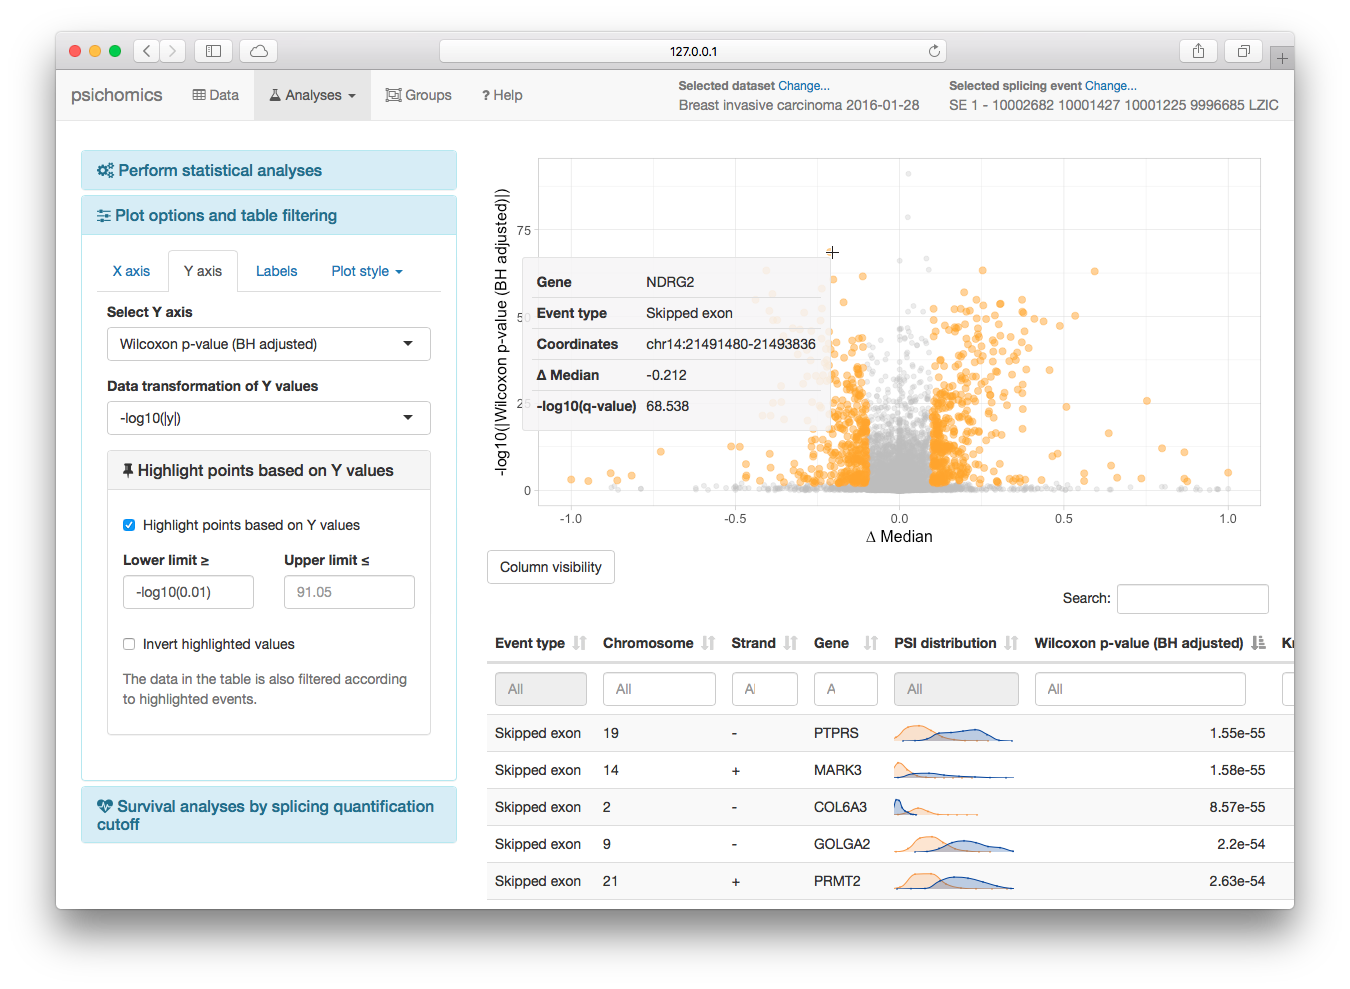
\includegraphics[width=.96\textwidth]{images/cTRAP/screenshot}
  \centering
  \vspace*{-.5cm}
  \caption[cTRAP global interface screenshot]{\textbf{cTRAP global interface screenshot} (21 Dec 2021).}
  \label{fig:cTRAP-screenshot}
\end{figure}

During a stormy day in our 2017 Madeira Lab retreat, we brainstormed the unique propositions of the lab that could most benefit the scientific community. One idea that emerged was to make it easier to identify putative causal perturbations by comparing the results of a custom differential gene expression analysis against the large-scale database of differential expression profiles from CMap \cite{subramanian:2017ul}, a repository of transcriptomic signatures for thousands of genetic (gene overexpression or knockout) and pharmacological perturbations of human cancer cell lines. % This kind of analysis is available in CMap's web apps at \alink{clue.io} \cite{subramanian:2017ul}, but their results are difficult to integrate in downstream analyses, suffer from poor API documentation for programatic access and lack basic visualisation tools.

% clue.io does indeed allow for batch query: https://clue.io/connectopedia/batch_query_tutorial
% clue.io API's is not straightforward: https://clue.io/connectopedia/query_api_tutorial

We thus developed cTRAP, an R package and web app to compare user-provided differential gene expression profiles with the perturbations available from CMap, allowing to infer putative candidate molecular causes for the observed differences, as well as compounds that may promote or revert them (\shortref{fig:cTRAP-screenshot}).

After releasing the first version in Bioconductor, multiple features were added (\shortref{tab:cTRAP}). Inspired by the method used to compare gene expression changes against the CMap database, we also added a way to predict drugs targeting altered genes by using datasets that featured both drug sensitivity and gene expression data for many cell lines. Additionally, cTRAP also allows to analyse the enrichment of molecular descriptor sets for compounds from NCI-60 and CMap. More recently, we developed a Shiny-based visual interface to host cTRAP online with support for user sessions and background tasks.

\begin{table}[!ht]
\parnotereset
\small
\caption[Major cTRAP milestones]{\textbf{Major cTRAP milestones.}}
\label{tab:cTRAP}
\begin{tabularx}{\textwidth}{ l r l }
\toprule
\textbf{Version} & \textbf{Release date} & \textbf{Main features} \\
\midrule
1.0  &  2 Nov 2018 & Compare differential expression profiles against CMap data\parnote{First Bioconductor release.} \\
\midrule
\multirow{3}*{1.4}  & \multirow{3}*{12 Nov 2019} & Predict targeting drugs using NCI-60, CTRP and GDSC data \\
       &             & Analyse enrichment for molecular descriptors of compounds \\
       &             & Load and process 21GB CMap z-scores file by chunks \\
\midrule
1.8  & 30 Oct 2020 & Include graphical functions to load data and analyse results \\
\midrule
\multirow{2}*{1.10} & \multirow{2}*{20 May 2021} & Improve speed and memory usage when comparing data \\
       &             & Set custom size for data chunks (1 GiB by default)  \\
\midrule
1.12 & 28 Oct 2021 & Add web server support (optimised to run in ShinyProxy)\parnote{First version available online.} \\
\bottomrule
\end{tabularx}
\parnotes
\end{table}

The associated cTRAP manuscript (of which I am a co-first and co-corresponding author) is in preparation for submission to an international peer-reviewed scientific journal and shares similarities with this chapter.

\section{Background}

Understanding the biological mechanisms underlying uncharacterised phenotypes is crucial to unravel the physiological role of genes and the mechanism of action of compounds, alongside their therapeutic potential \cite{subramanian:2017ul,malta:2018uj,mendez-lucio:2020th,le:2021uq,hughes:2000ww,almeida:2019wh}. Comprehending novel genetic and pharmacological perturbations -- including the modulation of the expression of a gene or induction of an unknown compound in a cellular system -- can be achieved by profiling genome-wide gene expression, allowing to analyse the whole cellular transcriptional response \cite{hughes:2000ww}.
% based on the assumption that cellular transcriptional response to pathway disruption is similar across cells, and that there are sufficiently unique transcriptional responses to the perturbation of most cellular pathways, systematic characterization of novel mutants could be carried out with a single genome-wide expression measurement

The gene expression profile of experimental phenotypic changes can be compared with a database of characterised transcriptomic signatures of known perturbagens, in order to infer putative molecular causes of the observed phenotype \cite{subramanian:2017ul,hughes:2000ww}. This approach requires a large, heterogeneous and representative dataset containing gene expression profiles associated with known perturbagens across multiple cell lines \cite{hughes:2000ww}. Such is the case of the Connectivity Map (CMap), a repository of transcriptomic signatures of thousands of genetic and pharmacological perturbations of human cancer cell lines \cite{subramanian:2017ul}. %Comparing differential gene expression profiles with those from CMap allows to infer putative molecular causes for the observed differences, as well as compounds that may promote or revert those changes.

CMap data can be explored and compared with user-provided data via a collection of user-friendly web apps from the CMap and LINCS Unified Environment (\mbox{\alink{clue.io}}) \cite{subramanian:2017ul}. However, \alink{clue.io} limits the maximum number of input genes for CMap queries (150 up-regulated and 150 down-regulated genes), %expresses results' significance in a non-standard significance score,
is difficult to automate for downstream analyses and cannot be run using local computing resources. Furthermore, \alink{clue.io} does not currently integrate with drug sensitivity datasets to further assist in pinpointing compounds that selectively target cells \cite{almeida:2019wh}.

\begin{figure}[!b]
  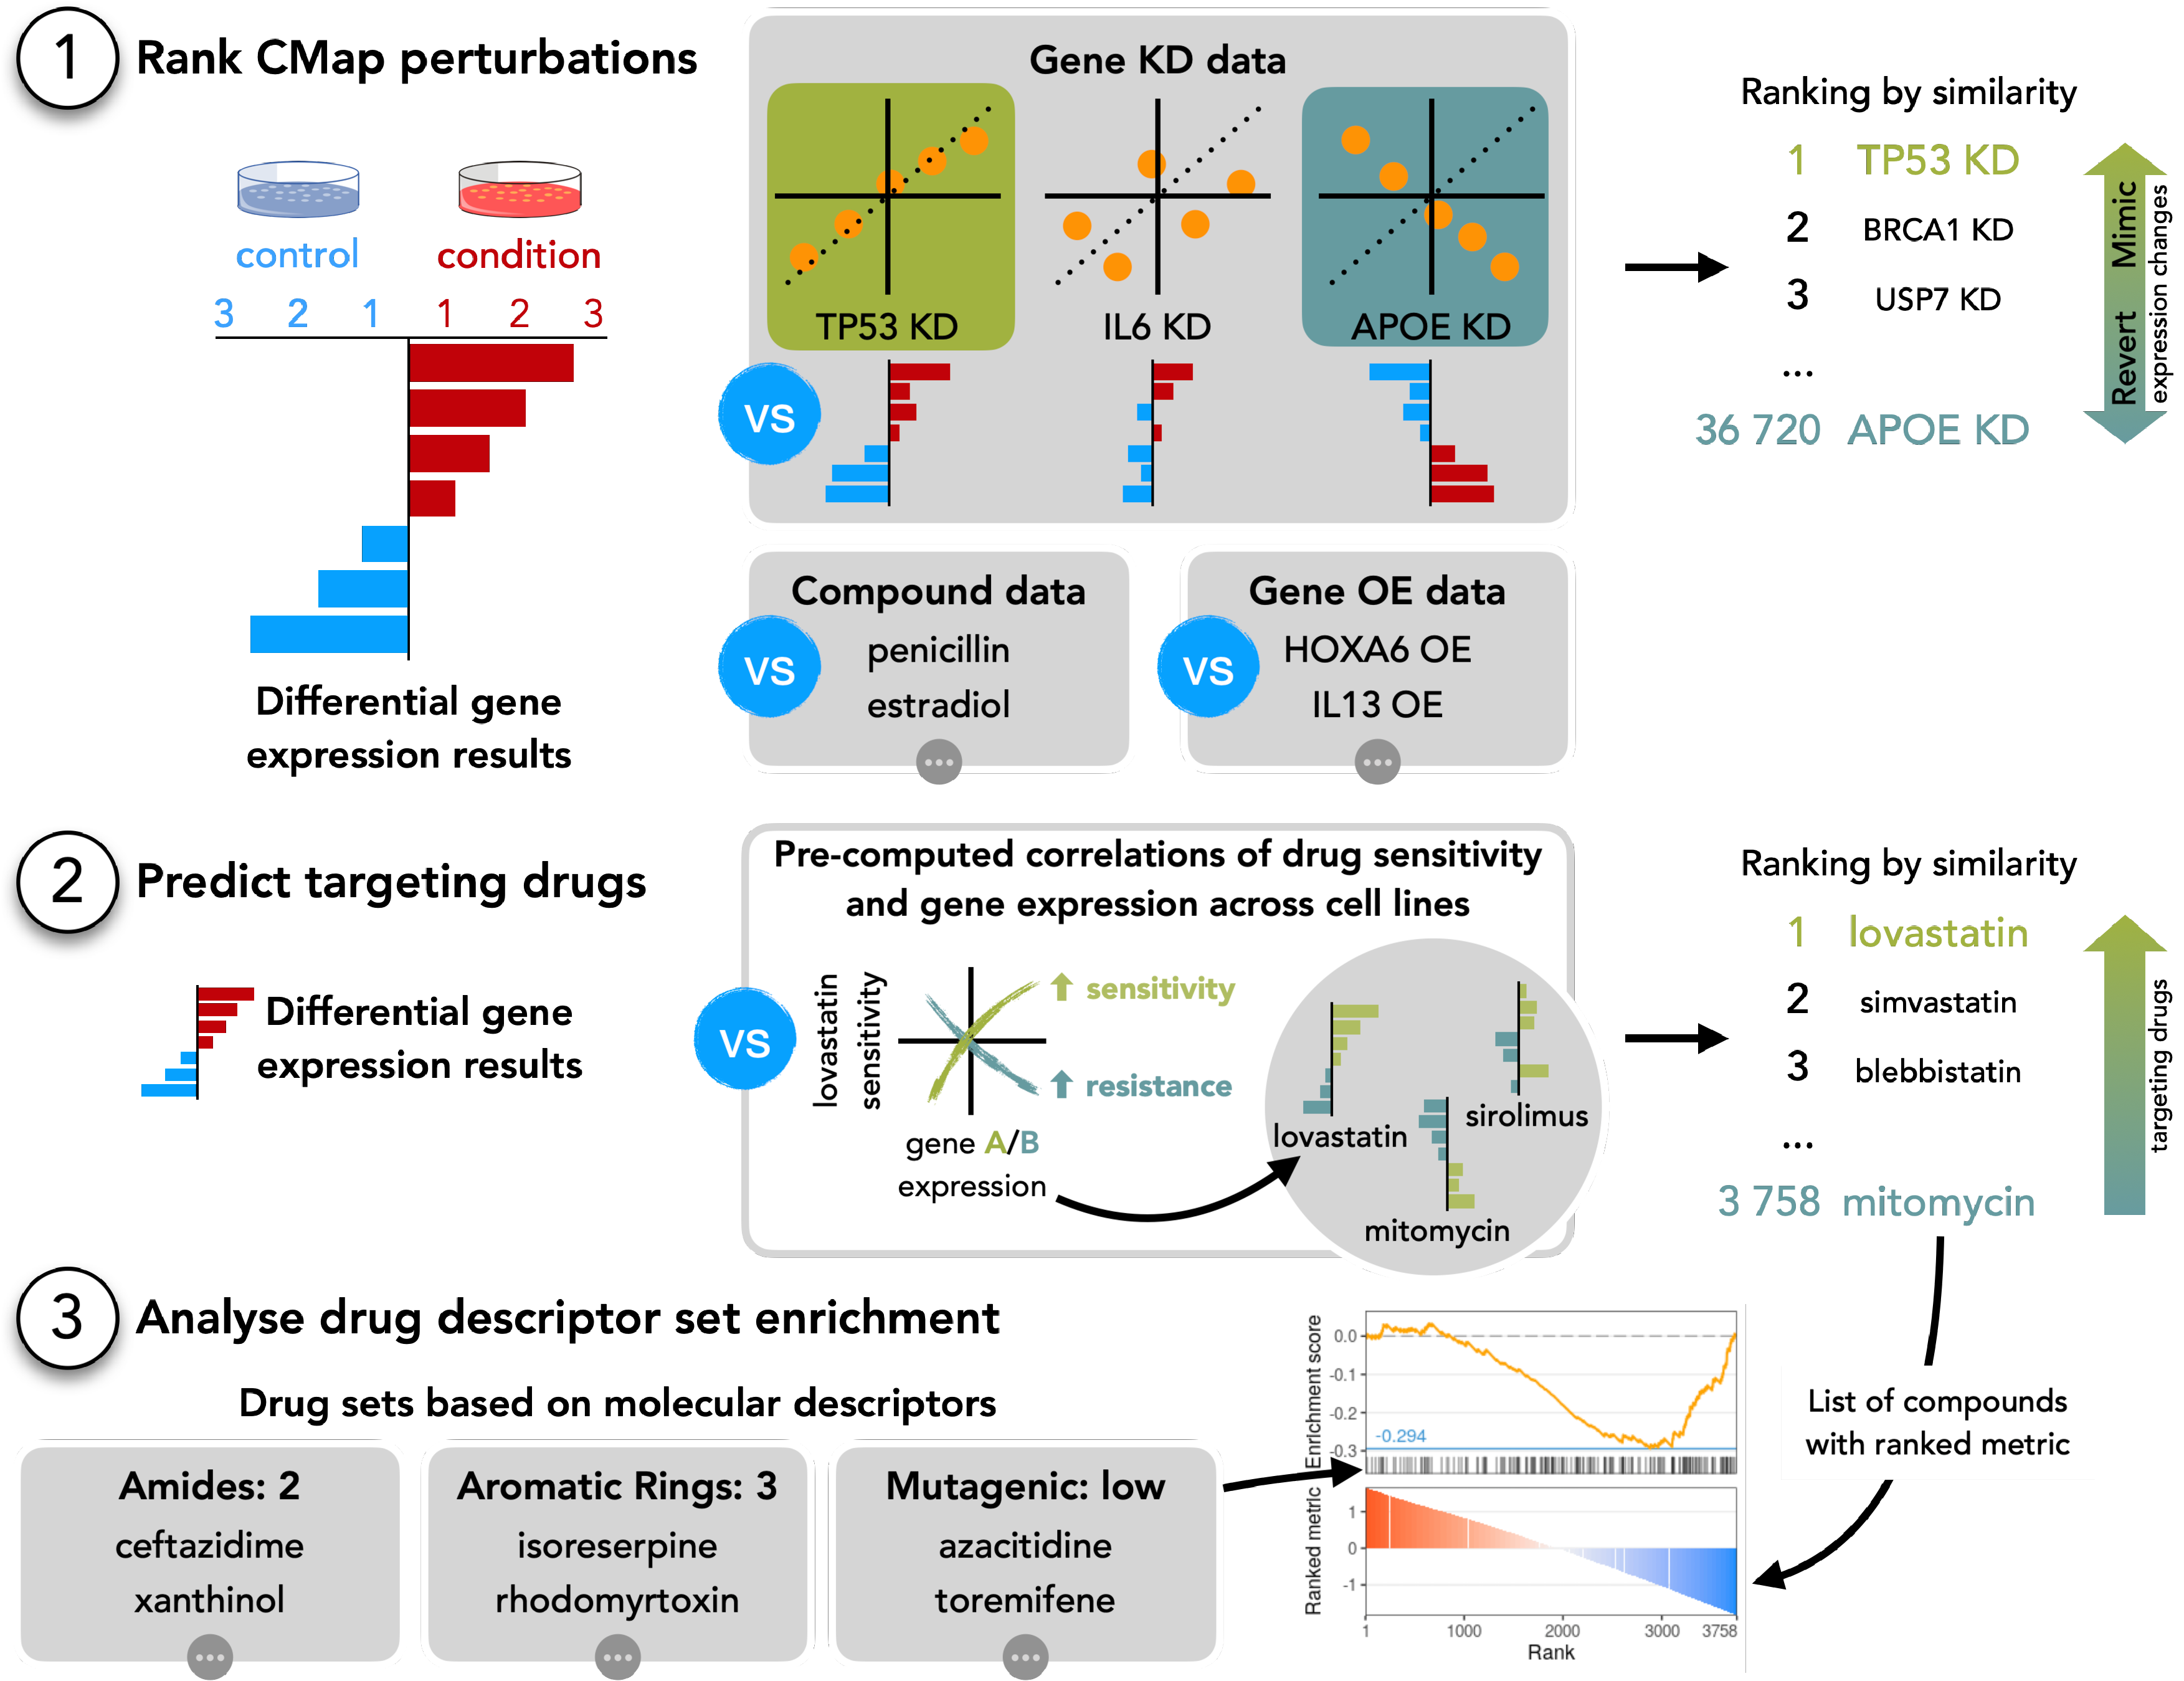
\includegraphics[width=\textwidth]{images/ctrap/ctrap}
  \centering
  \caption[cTRAP analyses]{\textbf{cTRAP analyses.} cTRAP allows to perform three types of analyses: \textbf{(1) rank CMap perturbations} based on the similarity between their associated gene expression alterations and user-provided differential gene expression values, \textbf{(2) predict targeting drugs} by comparing user-provided differential gene expression values with matrices of correlation between gene expression and drug sensitivity data across human cell lines and \textbf{(3) analyse drug descriptor set enrichment} (v. main text) using the compound list from either the first or second analysis.}
  \label{fig:ctrap}
\end{figure}

We thus developed cTRAP (\shortref{fig:ctrap}), an R package and web app that identifies potentially causal molecular perturbations by seamlessly comparing user-provided differential gene expression results with those available from CMap. cTRAP also supports comparisons with gene expression/drug sensitivity associations derived from the NCI-60 \cite{shoemaker:2006wi}, the Cancer Therapeutics Response Portal (CTRP) \cite{seashore-ludlow:2015ws} and the Genomics of Drug Sensitivity in Cancer (GDSC) \cite{yang:2012vk}, to identify compounds that could target the phenotypes associated with the user-provided differential expression profiles \cite{almeida:2019wh}. In cTRAP, similarity between differential gene expression results is measured by gene set enrichment \cite{subramanian:2017ul,subramanian:2005wu} and correlation scores. Finally, cTRAP can also analyse a list of compounds resulting from previous analyses for the enrichment in sets of computed molecular descriptors (e.g., number of oxygen atoms or aromatic rings) from CMap and NCI-60 compounds, allowing to identify common chemical properties of compounds of interest.

cTRAP is available online as a web app at \alink{compbio.imm.medicina.ulisboa.pt/cTRAP}, but can be locally installed using Bioconductor (\alink{bioconductor.org/packages/cTRAP}) or Docker (\dockerlink{nunoagostinho/ctrap}). The source code of cTRAP is available at \alink{github.com/nuno-agostinho/cTRAP}.

\section{Materials and methods}

From a vector of user-provided differential expression results (e.g., t-statistic values) with respective gene symbols, cTRAP can return a list of CMap perturbations ranked by similarity or predict candidate drugs for targeting the associated phenotype. Moreover, cTRAP can also analyse the enrichment of drug sets in an ordered vector of compounds to identify common chemical characteristics (Figures \shorterref{fig:ctrap-workflow} and \shorterref{fig:ctrap-file-structure}).

\begin{figure}[!ht]
  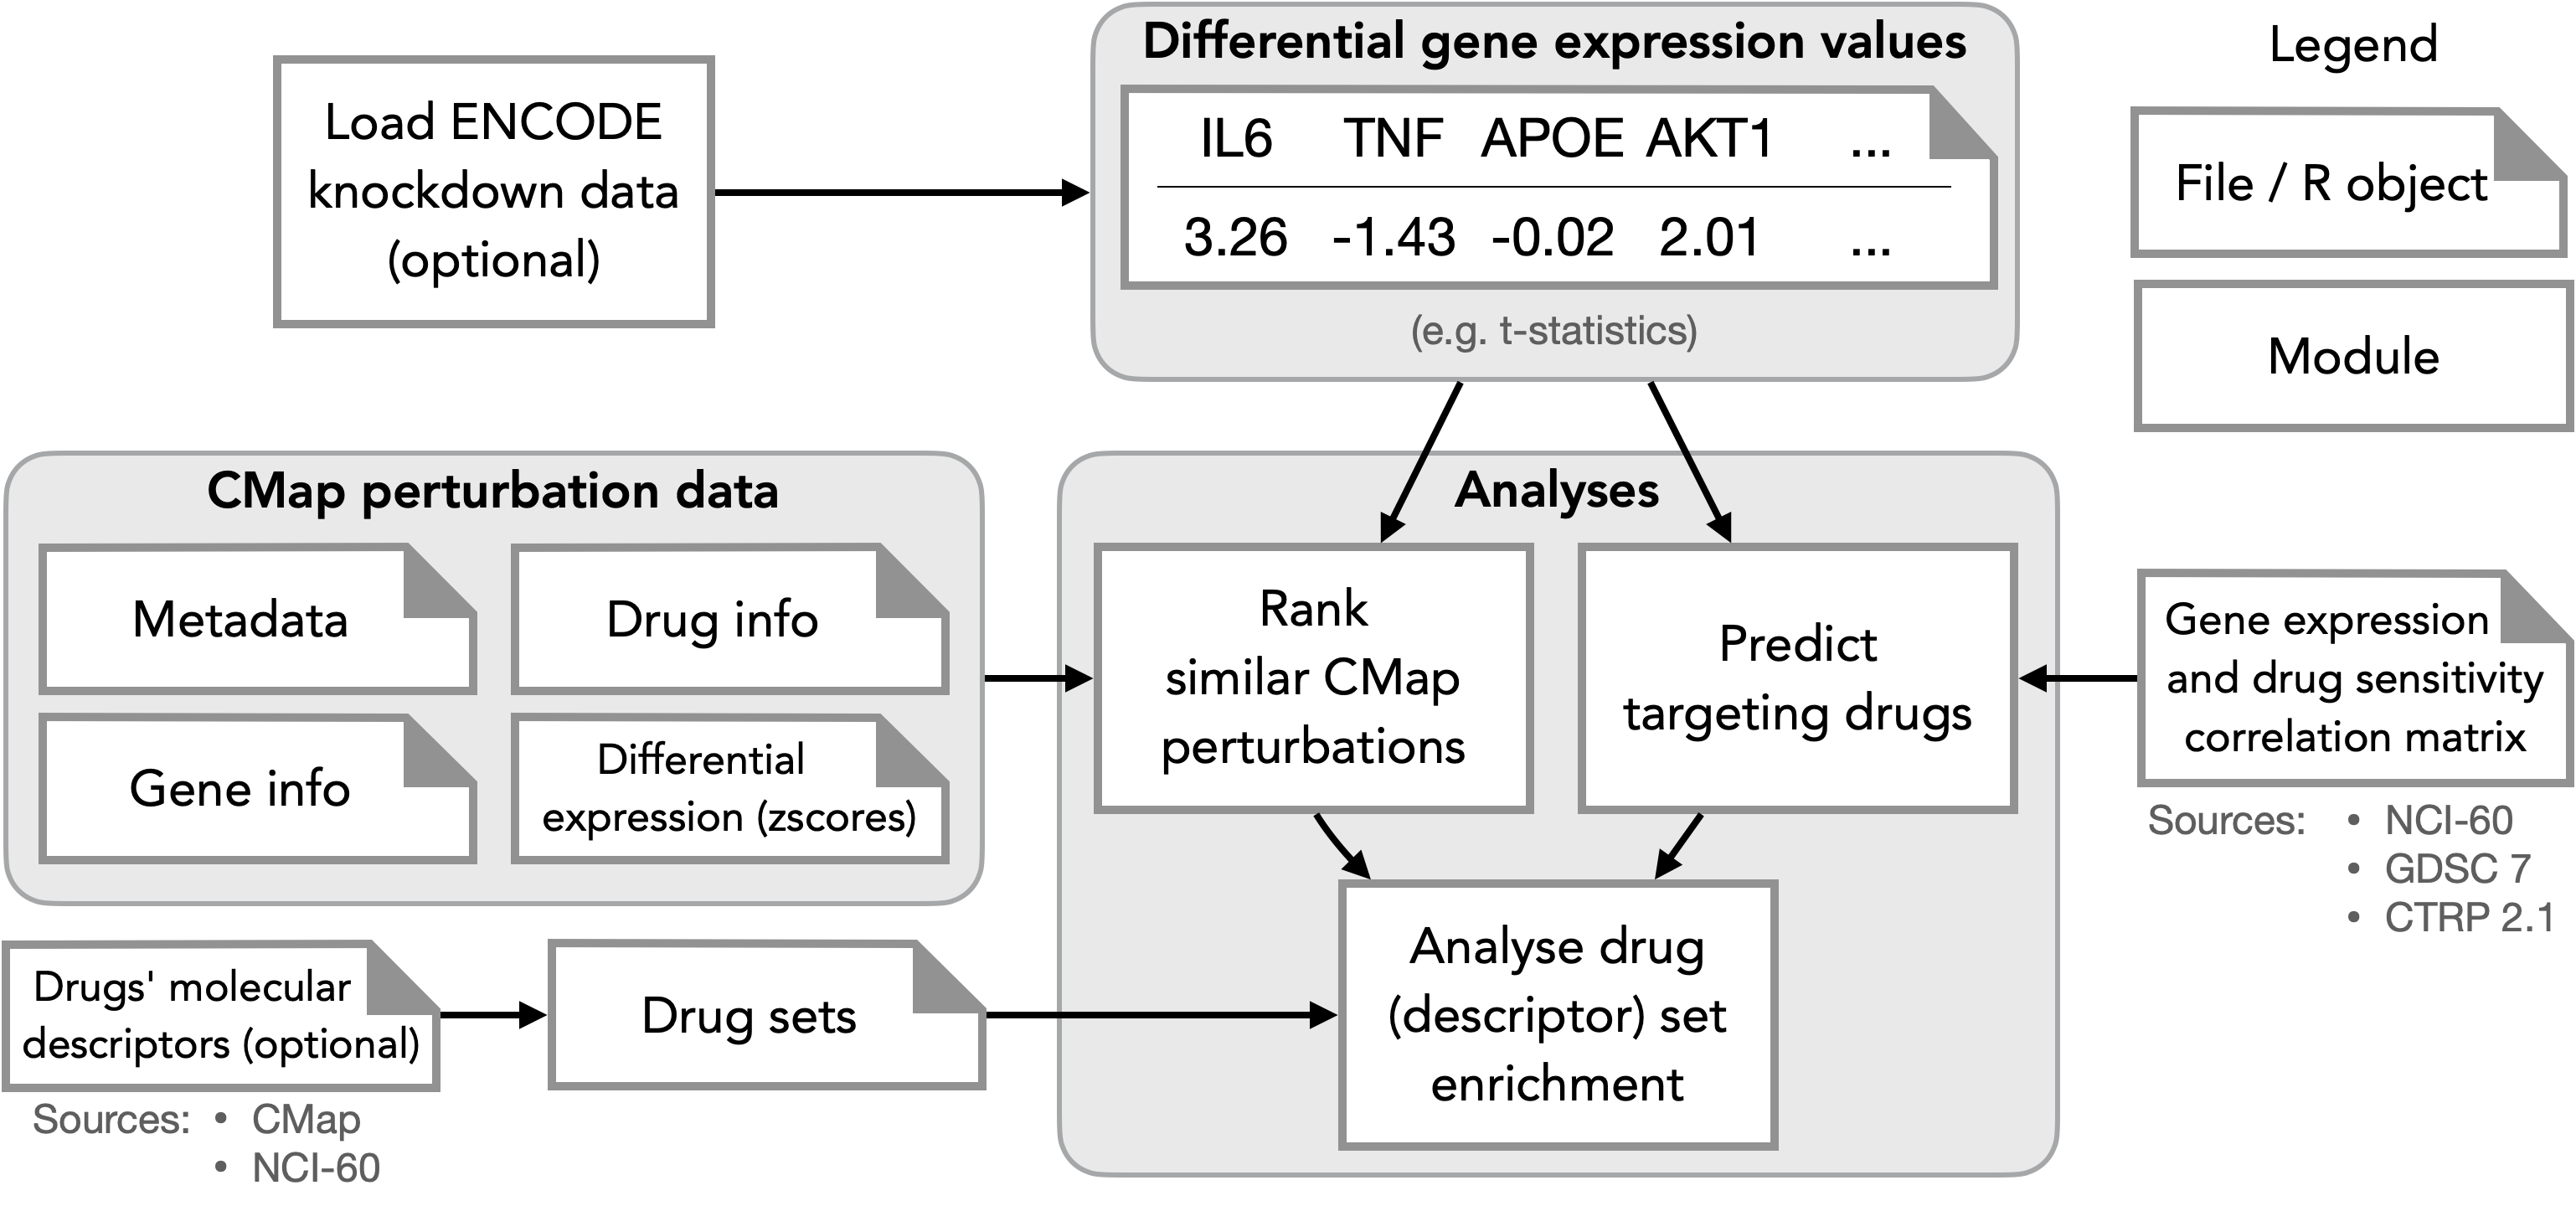
\includegraphics[width=.8\textwidth]{images/ctrap/workflow}
  \centering
  \caption[cTRAP workflow]{\textbf{cTRAP workflow.} A vector of differential gene expression values containing gene names is required to rank similar perturbations and to predict targeting drugs. Drug descriptor set enrichment analysis can then be performed based on those results. CMap perturbagen data, gene expression/drug sensitivity correlation matrices and molecular descriptors for drug sets can be automatically downloaded by cTRAP.}
  \label{fig:ctrap-workflow}
\end{figure}

\begin{figure}[!ht]
  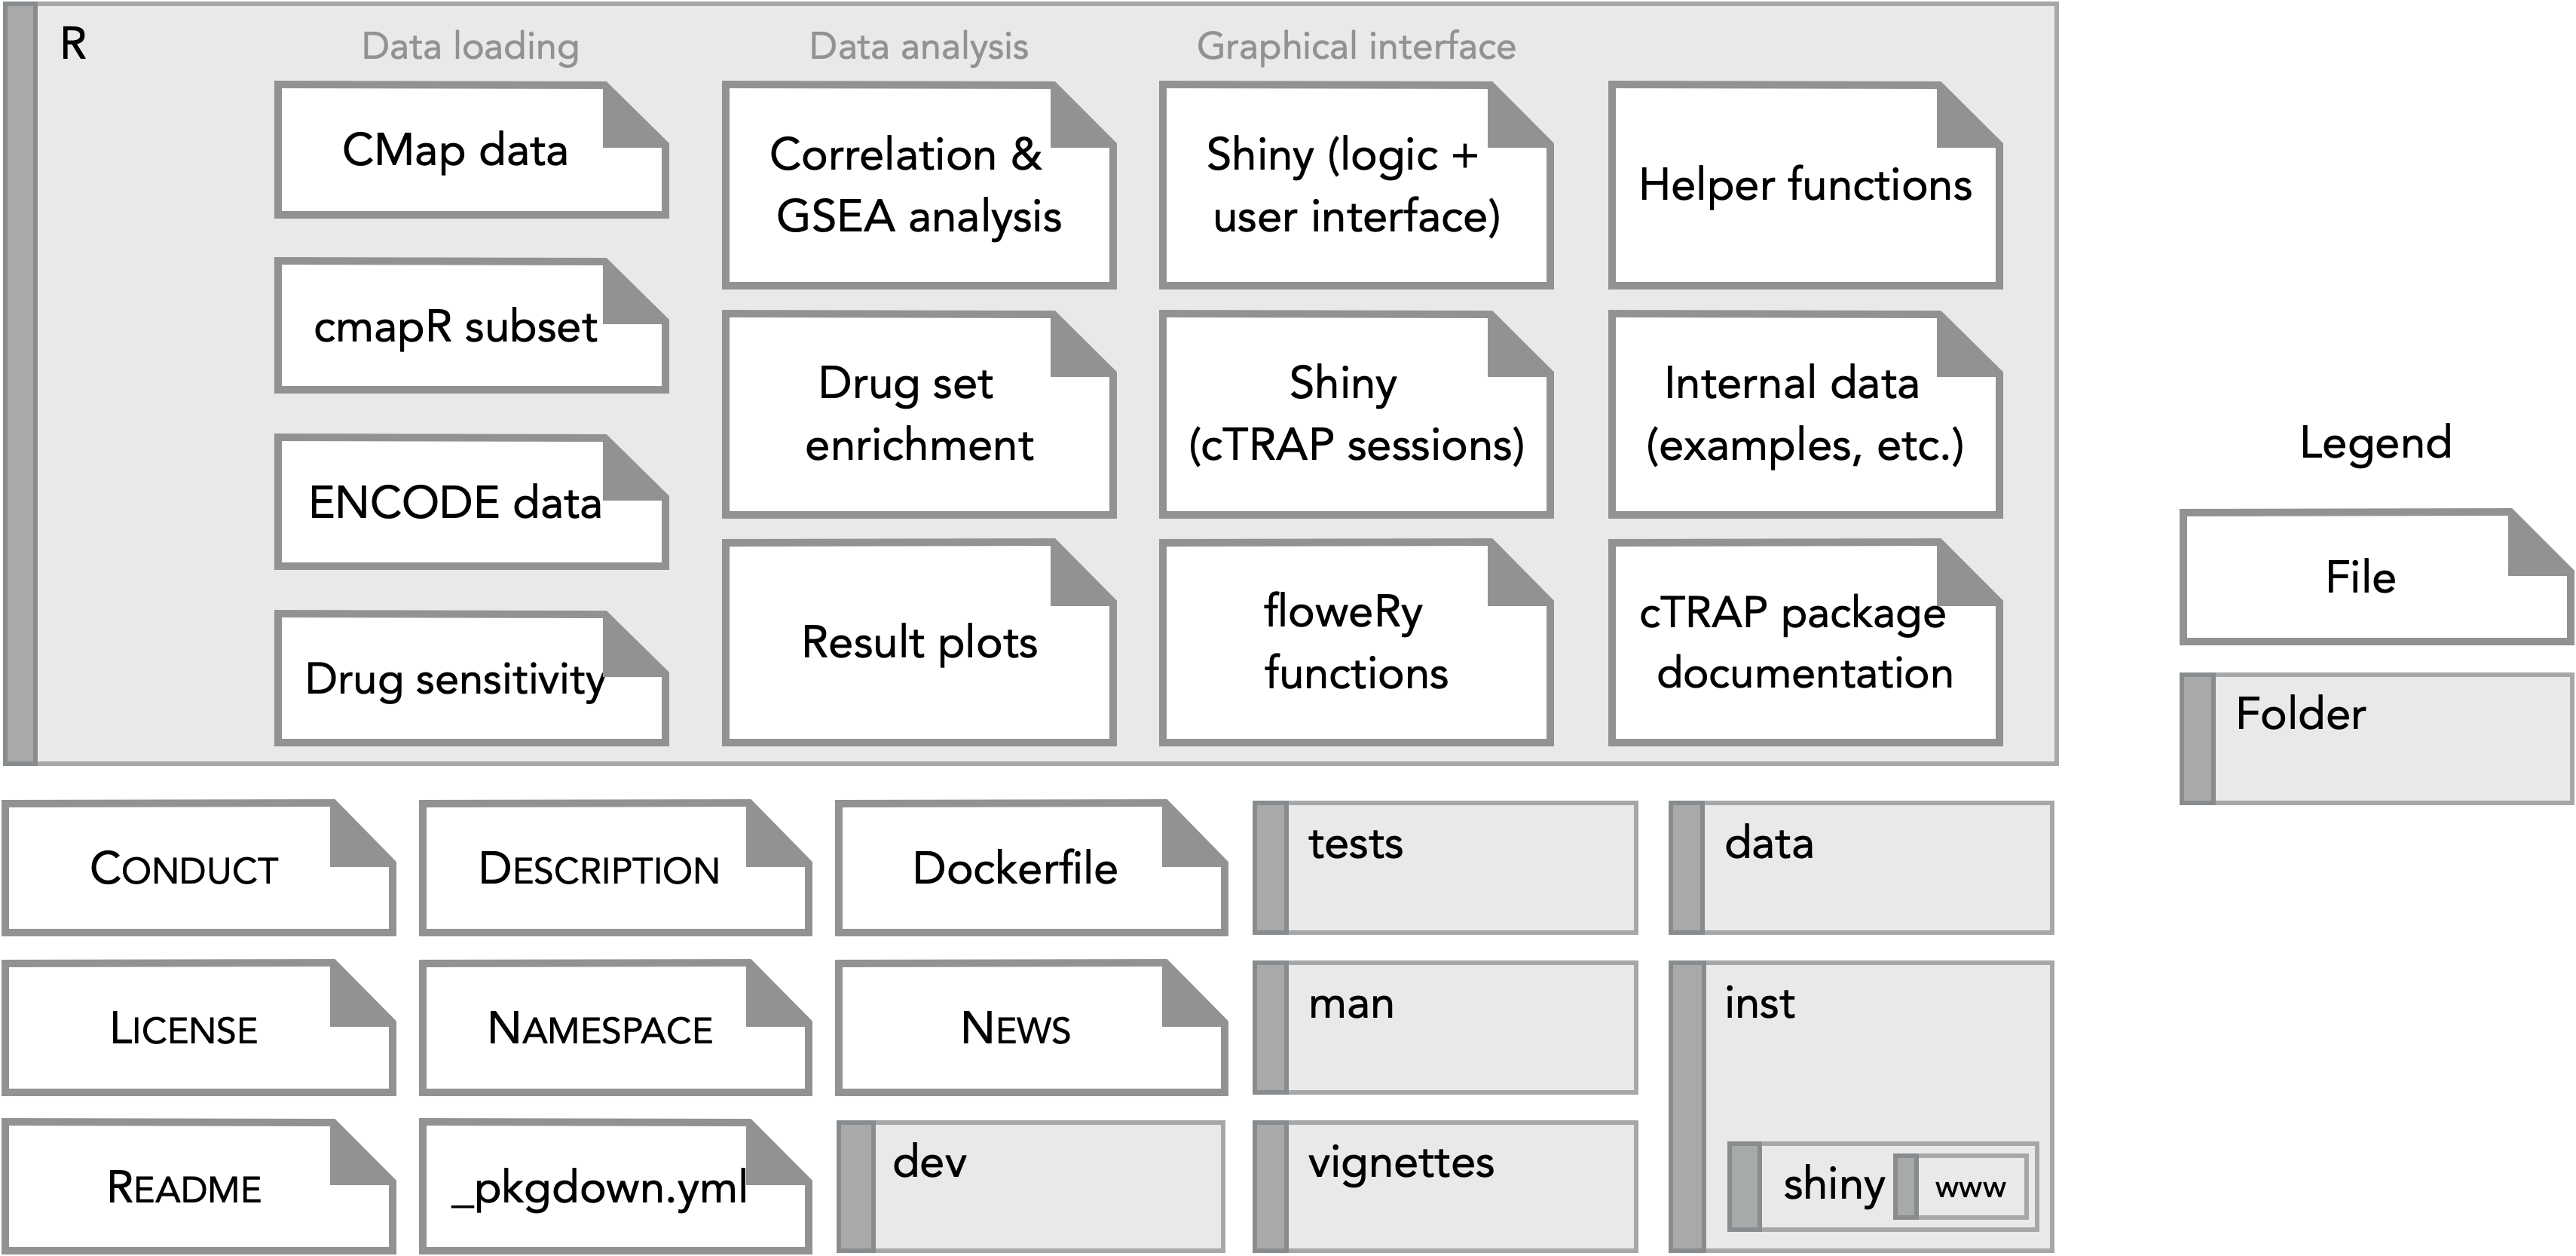
\includegraphics[width=1\textwidth]{images/ctrap/file-structure}
  \centering
  \caption[cTRAP file structure]{\textbf{Visual representation of cTRAP's file structure.} As usual in an R package, the \texttt{R} folder contains the scripts with cTRAP functions and data. \texttt{dev} is a custom folder that stores supporting scripts (e.g., test workflows and benchmarks); its contents are not included when building the R package.}
  \label{fig:ctrap-file-structure}
\end{figure}

\subsection{ENCODE knockdown data}

Using cTRAP, we can query and download ENCODE knockdown (and respective control) samples \cite{luo:2019tp} for multiple cell lines, filter genes/samples with low coverage from gene expression data, convert from ENSEMBL gene identifiers to gene symbols, and perform differential gene expression analysis using \texttt{voom()}, \texttt{lmFit()} and \texttt{eBayes()} from the \texttt{limma} R package \cite{ritchie:2015tm}. First, \texttt{voom()} is used with the \emph{quantile} normalisation to transform count data to log\textsubscript{2} CPM (counts per million) and estimate the mean-variance relationship to compute weights used in linear modelling. Gene-wise linear models are then fitted using \texttt{lmFit()} between the knockdown and the control samples, followed by moderated t-tests and the calculation of log-odds of differential expression, using \texttt{eBayes()} for empirical Bayes moderation of standard errors.

cTRAP includes an example dataset (\texttt{diffExprStat}) with the differential gene expression results (t-statistic values) associated with \emph{EIF4G1} knockdown in HepG2 cells (\shortref{lst:diffExprStat}).

\begin{lstlisting}[caption=Code to obtain example dataset \texttt{diffExprStat}.,language=R,label={lst:diffExprStat}]
library(cTRAP)
ENCODEmetadata <- downloadENCODEknockdownMetadata(cellLine="HepG2",
                                                  gene="EIF4G1")
ENCODEsamples  <- loadENCODEsamples(ENCODEmetadata)[[1]]
counts         <- prepareENCODEgeneExpression(ENCODEsamples)

# Remove low coverage genes (>= 10 counts shared by >= 2 samples)
minReads   <- 10
minSamples <- 2
filter     <- rowSums(counts[ , -c(1, 2)] >= minReads) >= minSamples
counts     <- counts[filter, ]

# Convert ENSEMBL identifiers to gene symbols
counts$gene_id <- convertGeneIdentifiers(counts$gene_id)

# Perform differential gene expression (DGE) analysis
diffExpr <- performDifferentialExpression(counts)

# Get t-statistic values of DGE and respective gene names
diffExprStat <- diffExpr$t
names(diffExprStat) <- diffExpr$Gene_symbol
\end{lstlisting}

\subsection{Ranking of similar CMap perturbations}

\begin{figure}[!b]
  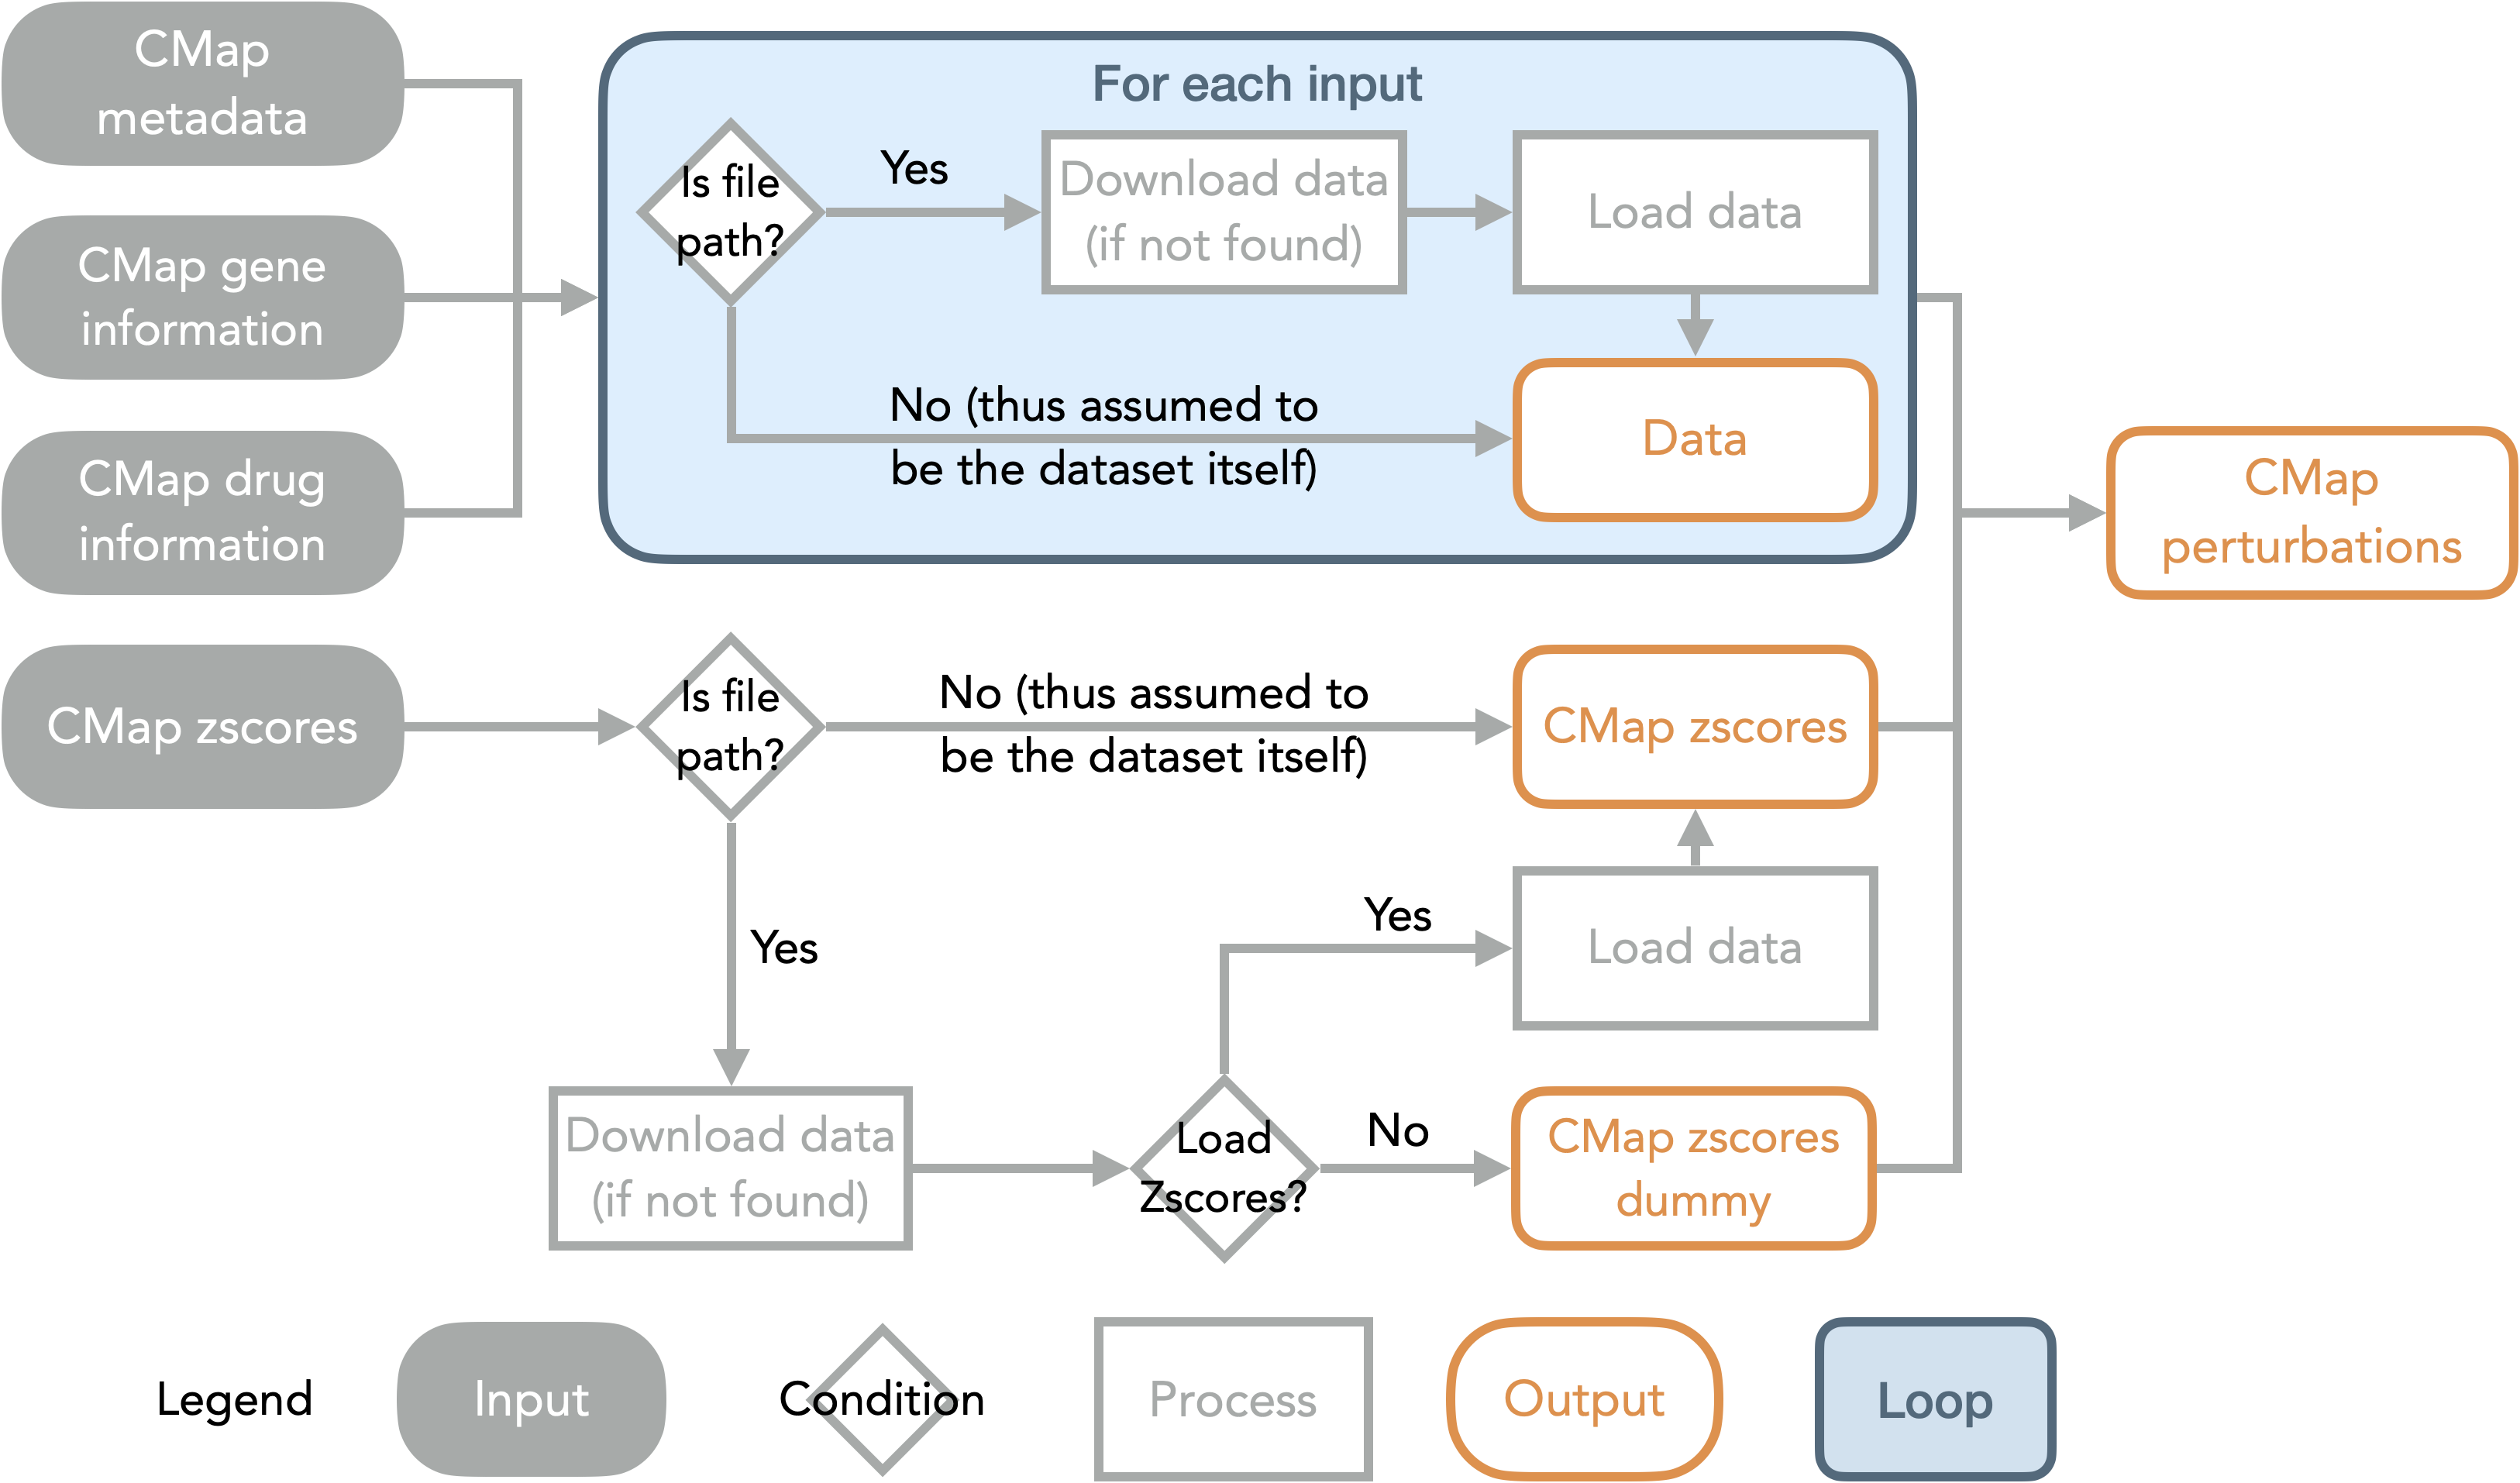
\includegraphics[width=.8\textwidth]{images/ctrap/cmap-perturbations}
  \centering
  \caption[Loading data from CMap perturbations]{\textbf{Loading data from CMap perturbations.} Input arguments support either the data themselves (as data frames) or their respective file path. If the file path directs to a non-existing file,  data are first downloaded and then saved to the given file path. To avoid high memory usage, CMap perturbations' differential expression z-scores (CMap zscores) are not loaded into memory when a file path is given. Instead, only metadata are loaded into a \emph{dummy} object that can be subset as a normal R object for downstream analyses.}
  \label{fig:ctrap-cmap-perturbations}
\end{figure}

CMap perturbations can be categorised into gene knockdown, gene over-expression and compounds. In cTRAP, available perturbation types and respective conditions can be enquired using the function \texttt{getCMapConditions()} that will download CMap perturbation metadata. Afterwards, \texttt{filterCMapMetadata()} allows to filter the metadata based on selected perturbations types, cell lines, dosages and time points, allowing to specifically load only the desired data in downstream analyses. This information is passed to \texttt{prepareCMapPerturbations()} to download (if file is not found) and process CMap differential expression normalised z-scores (GCTX file) and gene and compound information (\shortref{fig:ctrap-cmap-perturbations}). Given that the GCTX file size is around 21GB, we recommend to download the file directly from GEO GSE92742’s Level 5 data link (\sloppy{\small{\url{ftp://ftp.ncbi.nlm.nih.gov/geo/series/GSE92nnn/GSE92742/suppl/GSE92742_Broad_LINCS_Level5_COMPZ.MODZ_n473647x12328.gctx.gz}}}).

After comparing differential expression normalised z-scores from select CMap perturbations against user-provided differential expression results, \texttt{rankSimilarPerturbations()} returns a table with ranked CMap perturbations. Ranks closer to the top indicate perturbations whose differential expression profiles are more similar to the user-provided data, i.e., CMap perturbations that potentially mimic the user-provided transcriptomic changes, whereas higher ranks define perturbations that may revert those changes.

To rank CMap perturbations, cTRAP performs Spearman's and Pearson's correlations between the user-provided statistics for differential expression and values from CMap perturbations, and calculates a GSEA-based score (described below). All three methods are run by default. For each method, the similarity scores are averaged across multiple cell lines for the same conditions (i.e., same exposure time, dose and induced compound or gene target) and those averages are then used to rank CMap perturbations. By default, results for individual cell lines are provided for informative purposes (e.g., to check the heterogeneity of response across cell lines) but not used when ranking. The different ranking scores are combined via the rank product \cite{breitling:2004aa}, ultimately used to sort the CMap perturbations. % rank product not properly explained

The GSEA-based score is calculated via the following steps:

\begin{enumerate}
	\item Order genes by the user-provided differential expression statistics.
	\item Define the top 150 (by default) and bottom 150 (by default) genes as two sets.
	\item For each CMap perturbation, sort genes by their differential expression z-scores and calculate the Weighted Connectivity Score (WTCS), a composite and bi-directional version of the weighted Kolmogorov-Smirnov enrichment statistic (ES) \cite{subramanian:2017ul} where GSEA is run for the most up- and down-regulated genes from the user’s differential expression profile. The WTCS is the mean between $\textrm{ES}_{\textrm{top}}$ and $\textrm{ES}_{\textrm{bottom}}$; however, $\textrm{WTCS} = 0$ if both sets have the same sign \cite{subramanian:2017ul}.
\end{enumerate}

As an example, for a CMap perturbation with a similar differential expression profile to user’s input, we expect to find higher enrichment of the top gene set in the most up-regulated genes and higher enrichment of the bottom gene set in the most down-regulated genes.

To minimise peak RAM usage, \texttt{prepareCMapPerturbations()} downloads the GCTX file (a customised HDF5 file) for the CMap’s perturbation differential expression z-scores (if not previously downloaded) and returns its path without loading the file content itself, creating a \emph{dummy} object that only stores its file path, perturbation names, gene symbols and other associated metadata (\shortref{fig:ctrap-cmap-perturbations}). Based on the file path of this \emph{dummy} object (that can be subset like a normal R object), \texttt{rankSimilarPerturbations()} loads a $\le$ 1 GiB chunk\footnote{The default 1 GiB ($1024^3$ bytes) allows loading chunks of around 10000 columns and 14000 rows ($10000 \times 14000 \times 8 \textrm{ bytes} / 1024^3 = 1.04 \textrm{ GiB}$). CMap's GCTX file has around 14000 rows (genes).}, compares its differential expression z-score values against user-provided data and repeats the analysis for the next chunk (\shortref{fig:ctrap-analyses}). For each chunk, multithreaded support for Linux and macOS can be enabled per comparison method via \texttt{parallel::mclapply()}\footnote{\texttt{mclapply()} parallelises tasks via forking where multiple child processes are spawned and share their parent's memory. Forking is unavailable in Windows and its alternatives were deemed unsatisfactory, given that they copy 1GiB chunks per thread, significantly slowing down runtime.}, enabled by setting the number of threads to 2 or higher.

\begin{figure}[!ht]
  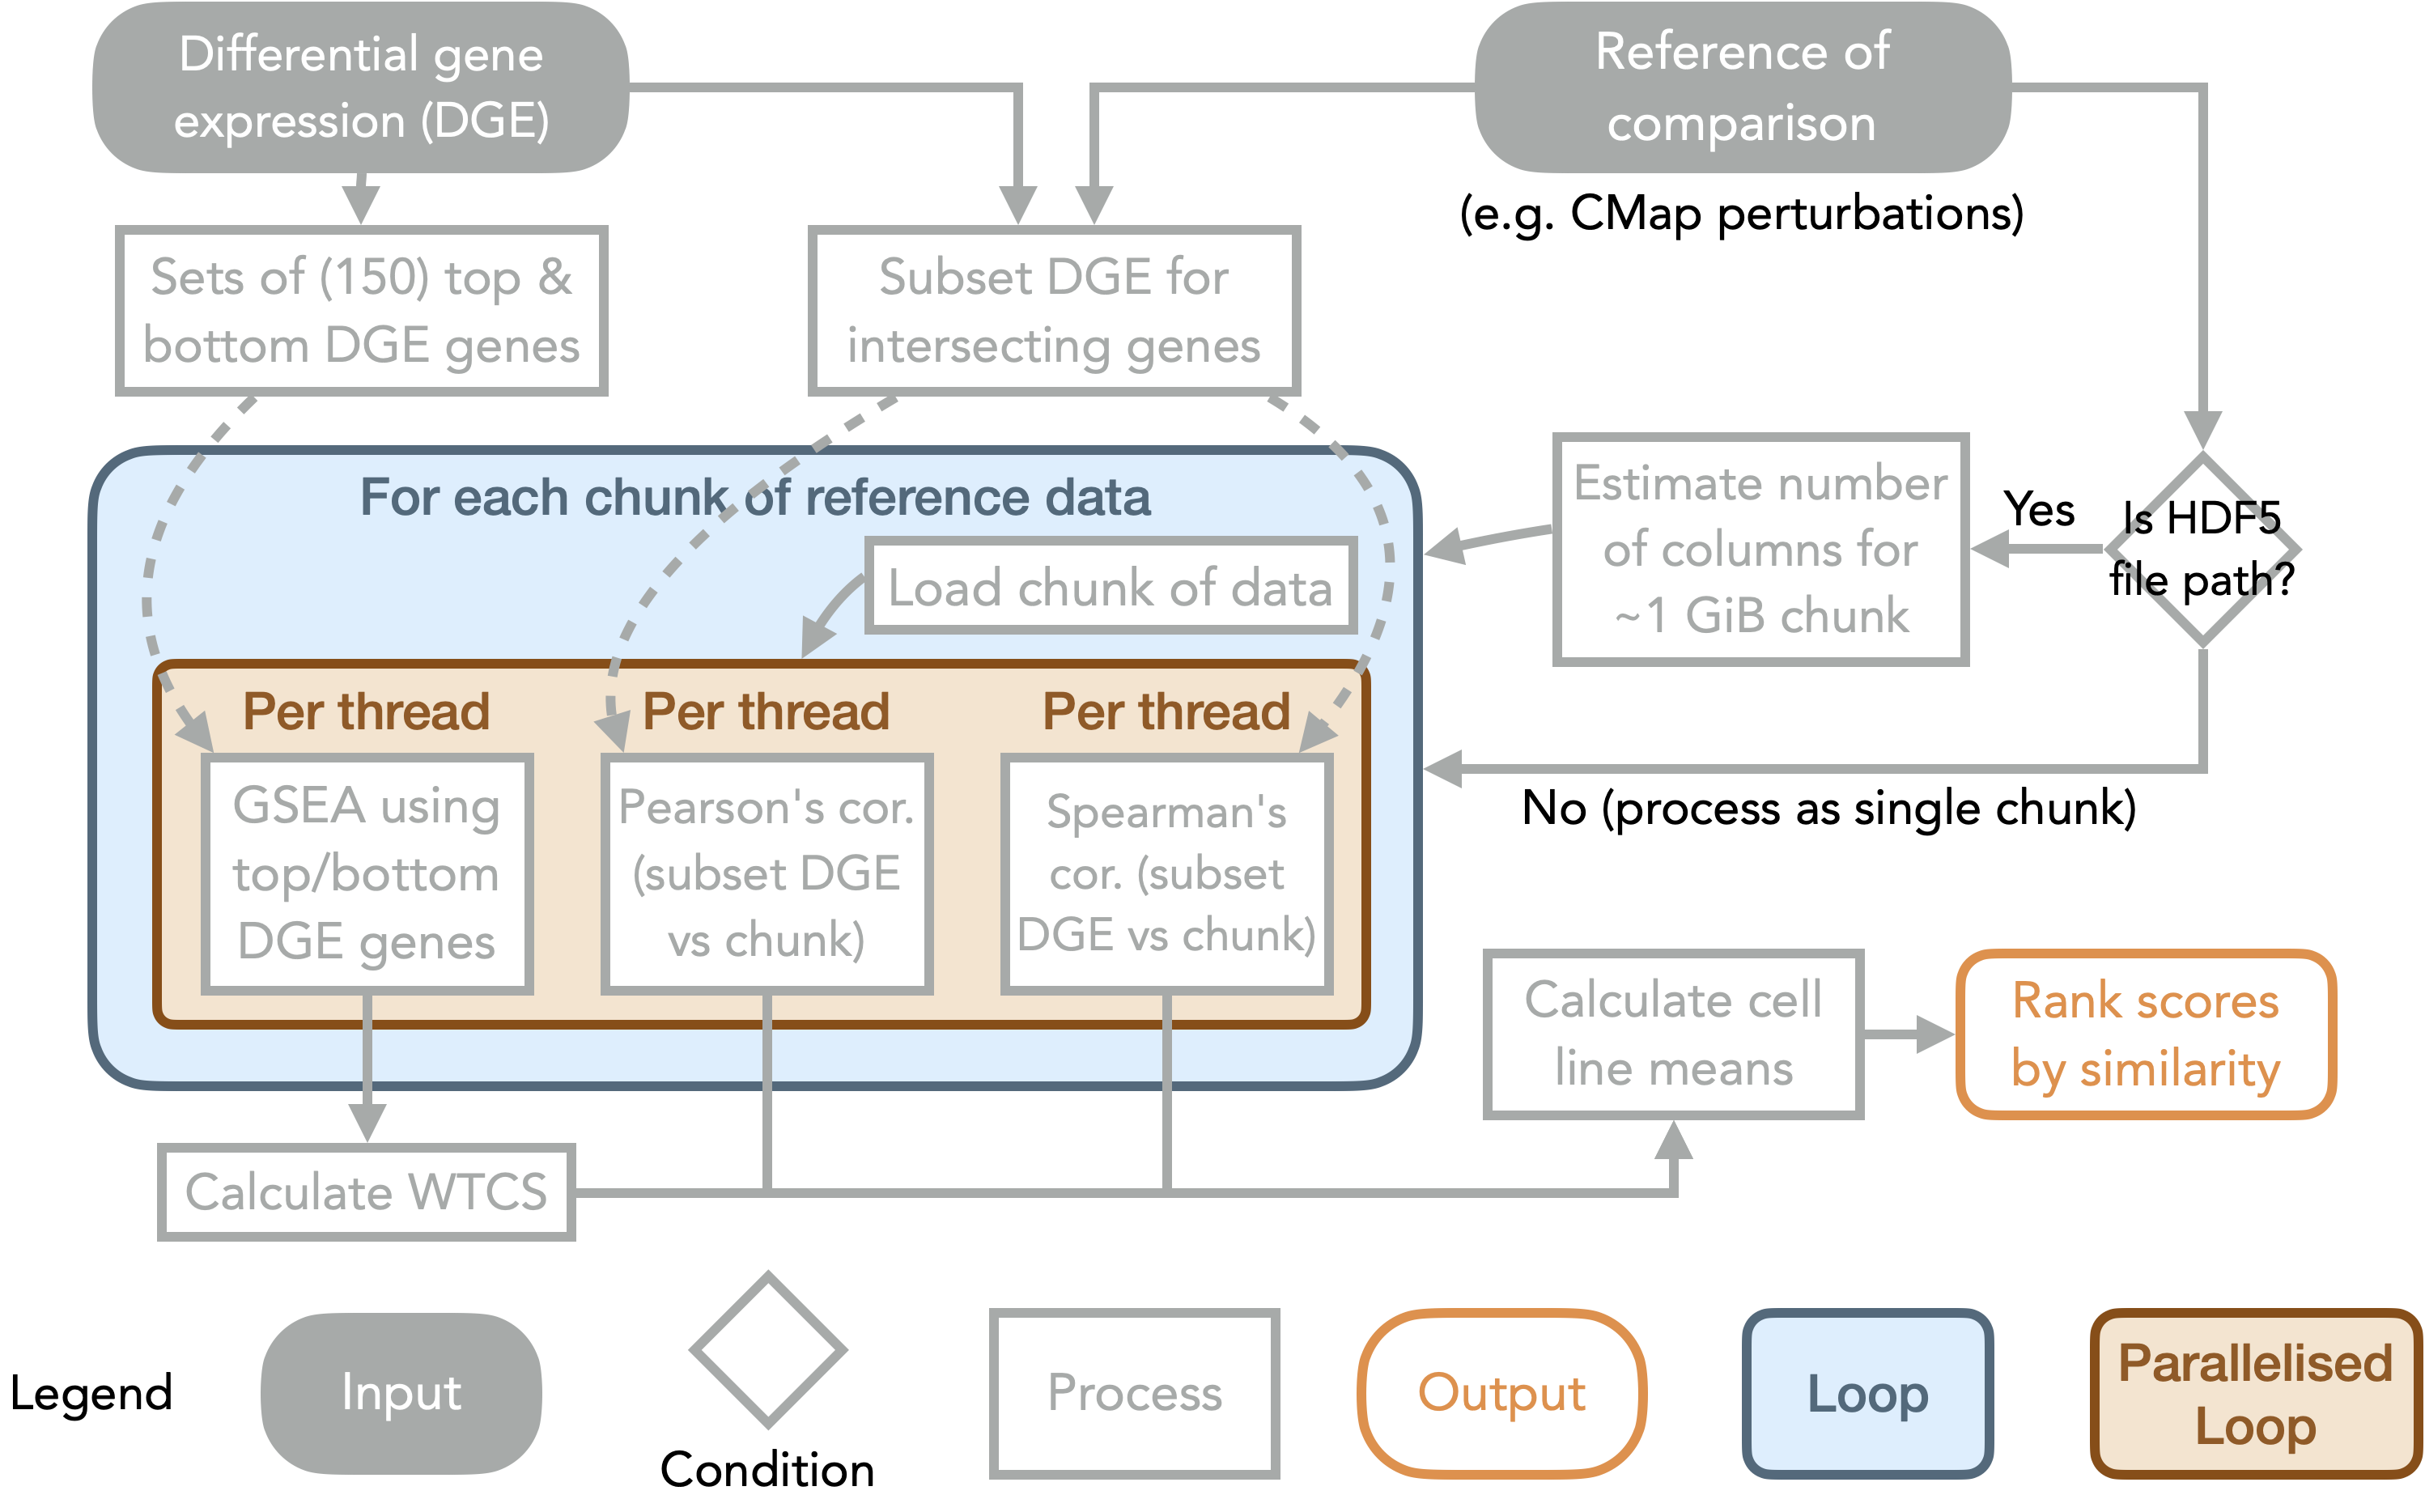
\includegraphics[width=.8\textwidth]{images/ctrap/analysis}
  \centering
  \caption[cTRAP similarity analysis]{\textbf{cTRAP similarity analysis.} User-provided differential gene expression statistics are compared with reference data (e.g., differential expression z-scores of CMap perturbations) and ranked by similarity. If the reference is contained in an HDF5 file, the file is processed in 1 GiB chunks (by default) to minimise peak memory usage. These analyses support multiple threads in Linux and macOS.}
  \label{fig:ctrap-analyses}
\end{figure}

The ranked list from \texttt{rankSimilarPerturbations()} can be plotted using \texttt{plot()}, showing a list of all results ordered by a given score or either a scatterplot or GSEA plot of the results for a single CMap perturbation (examples shown in \fullref{subsec:case-study}).

\pagebreak
\subsection{Prediction of targeting drugs}

Gene expression and drug activity data across multiple cell lines are available from NCI-60 \cite{shoemaker:2006wi}, Cancer Therapeutics Response Portal (CTRP) 2.1 \cite{seashore-ludlow:2015ws} and Genomics of Drug Sensitivity in Cancer (GDSC) 7 \cite{yang:2012vk} (\autoref{tab:drug-sensitivity-datasets}). For each source, the \texttt{prepareExpressionDrugSensitivityAssociation()} function performs the following:

\begin{enumerate}
	\item download all the necessary data depending on given source;
	\item perform Spearman’s correlation (by default) across cell lines between the expression of each gene and the sensitivity to each drug;
	\item generate a matrix with the correlation coefficients per gene and drug; and
	\item prepare metadata for downstream analyses, including gene, compound and cell line information from each source.
\end{enumerate}

As this process can take multiple hours to finish for all sources, the resulting objects were stored online for each aforementioned source and can be listed with \texttt{listExpressionDrugSensitivityAssociation()} and downloaded and loaded into R using \texttt{loadExpressionDrugSensitivityAssociation()}.

A positive correlation coefficient for a given gene and drug suggests a gene whose expression is associated with sensitivity to that drug across multiple cell lines. By calculating the susceptibility of genes for each annotated drug, we can then correlate this information with a given phenotype to rank compounds based on their potential to selectively target the queried (or similar) phenotypes, i.e., to selectively target phenotypes characterised by the overexpression of genes conferring susceptibility to the compounds.

\begin{wraptable}{r}{7cm}
\centering
\parnotereset
\small
\caption[Drug sensitivity datasets statistics]{\textbf{Drug sensitivity dataset statistics.} Number of screened compounds and human cancer cell lines available in cTRAP datasets.}
\label{tab:drug-sensitivity-datasets}
\begin{tabularx}{.45\textwidth}{ l r r }
\toprule
\textbf{Source}   & \textbf{Compounds} & \textbf{Cell lines} \\
\midrule
NCI-60            &             21 738 &   60 \\
GDSC 7            &                266 &  983 \\
CTRP 2.1          &                545 &  823 \\
\bottomrule
\end{tabularx}
\parnotes
\end{wraptable}

To identify compounds that could target the phenotype associated with specific differential expression profiles, we use \texttt{predictTargetingDrugs()} with those profiles and a correlation matrix of gene expression and drug sensitivity as input. The correlation coefficients between gene expression and drug sensitivity for each drug are compared against user-provided differential expression results by Spearman’s and Pearson’s correlation and WTCS (as performed when ranking CMap perturbations, results from comparison methods are ranked and then those rankings are finally used to calculate the rank product’s rank). \texttt{predictTargetingDrugs()} returns a table with ranked predicted targeting drugs and their respective correlation coefficients and WTCS (\shortref{fig:ctrap-analyses}). The ranks closer to the top comprise drugs that may target phenotypes similar to the user-provided differential expression profile.

The resulting object can be plotted with \texttt{plot()}, showing a list of all results ordered by a given score or either plots for a single predicted targeting drug. The function \texttt{plotTargetingDrugsVSsimilarPerturbations()} compares the results from predicted targeting drugs and CMap perturbations that may mimic or revert the observed phenotype. For the available compound identifiers in the metadata pertaining from the different datasets (e.g., compound name, Broad ID, PubChem CID and SMILES), the function will automatically select the identifiers with higher number of matching values between the two datasets, unless the identifiers are explicitly defined by the user. A scatterplot is then returned using, by default, the rank product’s rank of targeting drugs against the rank product’s rank of similar perturbations (examples shown in \fullref{subsec:case-study}).

\subsection{Drug descriptor set enrichment analysis}
\label{subsec:descriptor-set-enrichment}

Juan Carlos, a former member of the lab, computed drug descriptors (e.g., molecu\-lar weight and number of aromatic rings) for compounds from CMap and NCI-60 based on their three-dimensional (3D) and two-dimensional (2D) characteristics. These descriptors were uploaded to \alink{compbio.imm.medicina.ulisboa.pt/public/cTRAP/} and the resulting files can be automatically downloaded and processed to R using \texttt{loadDrugDescriptors()}.

\texttt{prepareDrugSets()} allows to create sets of descriptors. By default, the function creates a maximum of 15 sets per drug descriptor. For each alphanumeric descriptor, one set is created per unique value of that descriptor. Alphanumeric descriptors containing more than 15 unique values (by default) will be discarded. For numerical descriptors, \texttt{prepareDrugSets()} internally uses the \texttt{binr::bins()} function to create evenly-distributed bins of drug descriptors, where each set contains a minimum number of points equal to the number of non-missing values divided by the number of maximum sets (15 by default) divided by a constant (5 by default).

The \texttt{analyseDrugSetEnrichment()} function analyses the enrichment of the created drug descriptor sets in a named numeric vector or an object returned from \texttt{rankSimilarPerturbations()} or \texttt{predictTargetingDrugs()}. The GSEA-based enrichment analysis is internally performed using \texttt{fgsea::fgsea()} \cite{sergushichev:2016aa}. The resulting object can be plotted with \texttt{plot()}, showing a list of all results ordered by a given score or plots for a single predicted targeting drug.

\subsection{Time and memory benchmarking}

We measured elapsed time using R’s \texttt{Sys.time()} immediately before and after ranking similar CMap perturbations, predicting targeting drugs (using NCI-60 expression and drug sensitivity association, the most time-consuming option) and performing drug set enrichment analysis using a development version of cTRAP 1.10 (commit \link{https://github.com/nuno-agostinho/cTRAP/commit/296f9b2}{296f9b2} from January 2022). As input, we used the t-statistics for the differential expression between \emph{EIF4G1} knockdown versus control based on ENCODE gene expression data for cell line HepG2 (\texttt{cTRAP::diffExprStat} object).

Using the same input, we measured heap memory usage of cTRAP 1.10 dev (\link{https://github.com/nuno-agostinho/cTRAP/commit/296f9b2}{296f9b2}) while ranking CMap perturbations when running R 4.0.3 in debug mode with heaptrack 1.0.0\footnote{heaptrack is an open-source memory allocation profiler available at \alink{github.com/KDE/heaptrack}}. For R to work properly with heaptrack, the \path{/usr/bin/R} file was edited -- all lines of the last \emph{if} statement were commented out, except for:

\begin{lstlisting}[language=bash,numbers=none]
exec ${debugger} ${debugger_args} "${R_binary}" ${args} "${@}"
\end{lstlisting}

Afterwards, we benchmarked the memory usage while running cTRAP with:

\begin{lstlisting}[language=bash,numbers=none]
R -d heaptrack -f ${cTRAP_Rscript} --args ${cTRAP_Rscript_args}
\end{lstlisting}

All benchmarks were run in a workstation with Ubuntu 18.04.5 LTS, 768 GB of RAM memory and 72 cores (Intel Xeon Gold 6254 CPU @ 3.10GHz). The benchmark scripts are open-source and describe how to profile time and memory in cTRAP and plot subsequent results: \alink{github.com/nuno-agostinho/cTRAP/tree/master/dev/benchmark}.

\subsection{Continuous integration}

Akin to psichomics (\fullref{subsec:psichomics-ci}), GitHub Actions are used with cTRAP to update its Docker images in Docker Hub (\dockerlink{nunoagostinho/ctrap}) and GitHub (\alink{github.com/nuno-agostinho/cTRAP}); update website documentation via \texttt{roxygen} \cite{wickham:2021wt} and \texttt{pkgdown} \cite{wickham:2021wj}; and check for errors and warnins when building cTRAP in Windows, macOS and Linux.

\section{Results}

cTRAP's web app is available at \alink{compbio.imm.medicina.ulisboa.pt/cTRAP}. Alternatively, users can install cTRAP, allowing them to use local computing resources. Similarly to psichomics, cTRAP offers both graphical and command-line interfaces. Although most features are common to both interfaces, we recommend less experienced users to opt for the Shiny-based graphical interfaces.

\subsection{Case study}
\label{subsec:case-study}

To showcase cTRAP, we used RNA-seq data from \emph{EIF4G1} shRNA knockdown experiments in the HepG2 cell line from the ENCODE project \cite{luo:2019tp}. \emph{EIF4G1} (Eukaryotic Translation Initiation Factor 4 Gamma 1) encodes for the EIF4G1 scaffolding protein that contains binding sites for subunits of the EIF4F protein complex, required to initiate cap-dependent translation \cite{luo:2019tp,tu:2010vi,jaiswal:2018uq}. EIF4G1 is involved in cancer cell proliferation and migration and \emph{EIF4G1} knockdown has been suggested to impair tumourigenicity in prostate and epithelial cancer cells \cite{tu:2010vi,jaiswal:2018uq}.

Using cTRAP functions, we downloaded pre-processed gene quantification data for \emph{EIF4G1} knockdown (ENCFF955TXI and ENCFF049UZV, two replicates) and controls (ENCFF657KMW and ENCFF726AVT) from ENCODE \cite{luo:2019tp}. Afterwards, we quantilise-normalised the gene expression data with \texttt{voom} \cite{ritchie:2015tm} and performed differential expression analysis with \texttt{limma} \cite{ritchie:2015tm}.

\subsubsection{Comparison with CMap perturbations}

We compared ENCODE's t-statistic for the \emph{EIF4G1} knockdown expression changes against the normalised z-scores associated with CMap's knockdown and small molecule perturbations in HepG2\footnote{This comparison could also be performed to perturbations in a different cell line (or in all cell lines using the average result across cell lines).}. The comparisons were performed using Spearman's correlation, Pearson's correlation and WTCS (using the default 150 up-regulated and 150 down-regulated genes). All results were ordered based on the rank product's rank.

Within CMap knockdown perturbations, the top result is expectedly the knockdown of \emph{EIF4G1} in CMap data, working as a positive control (\autoref{tab:eif4g1-cmap-kd} and \autoref{fig:eif4g1-compound-plots}).

\begin{table}[!ht]
\centering
\footnotesize
\caption[Top 10 CMap HepG2 gene knockdown perturbations]{\textbf{Top 10 most similar CMap HepG2 gene knockdown perturbations} compared to \emph{EIF4G1} knockdown profile. Results ordered by rank product's rank. Legend: \emph{rho} is Spearman's coefficient and \emph{r} is Pearson's coefficient.}
\label{tab:eif4g1-cmap-kd}
\begin{tabular}{lllllllllllll}
\toprule
\textbf{Gene}     & \textbf{\emph{rho}} & \textbf{\emph{r}} & \textbf{WTCS} & \textbf{Gene description}                           \\
\midrule
\textbf{EIF4G1}   & 0.18         & 0.19       & 0.49          & eukaryotic translation initiation factor 4 gamma, 1 \\
\textbf{SKIV2L}   & 0.14         & 0.18       & 0.51          & Ski2 like RNA helicase                              \\
\textbf{MECP2}    & 0.19         & 0.18       & 0.39          & methyl-CpG binding protein 2                        \\
\textbf{KIF20A}   & 0.17         & 0.18       & 0.46          & kinesin family member 20A                           \\
\textbf{MEST}     & 0.17         & 0.19       & 0.42          & mesoderm specific transcript                        \\
\textbf{COPS5}    & 0.18         & 0.18       & 0.42          & COP9 signalosome subunit 5                          \\
\textbf{PPIH}     & 0.19         & 0.17       & 0.44          & peptidylprolyl isomerase H                          \\
\textbf{STAT1}    & 0.18         & 0.19       & 0.38          & signal transducer and activator of transcription 1  \\
\textbf{KIAA0196} & 0.19         & 0.18       & 0.35          & KIAA0196                                            \\
\textbf{SQRDL}    & 0.19         & 0.17       & 0.40          & sulfide quinone reductase-like (yeast)             \\
\bottomrule
\end{tabular}
\end{table}

\begin{figure}[!ht]
	\centering
	  \vspace{-\intextsep}
	\begin{subfigure}[h]{0.45\textwidth}
		\begin{overpic}[width=\textwidth]{images/ctrap/eif4g1-compound-plot-scatter}
			\put(1,85){\textsf{\textbf{a}}}
		\end{overpic}
	\end{subfigure}
	\begin{subfigure}[h]{0.45\textwidth}
		\begin{overpic}[abs,width=\textwidth]{images/ctrap/eif4g1-compound-plot-gsea}
			\put(.6,167){\textsf{\textbf{b}}}
			\put(.6,107){\textsf{\textbf{c}}}
			\put(.6,54){\textsf{\textbf{d}}}
		\end{overpic}
	\end{subfigure}
    \caption[Comparison of \emph{EIF4G1} knockdown in HepG2 between ENCODE and CMap]{\textbf{Comparison of the \emph{EIF4G1} knockdown experiments in HepG2 cells between ENCODE and CMap.} (a) Scatterplot of differential gene expression values of \emph{EIF4G1} knockdown for common genes between ENCODE (t-statistics; X-axis) and CMap (normalised z-scores; Y-axis). (b-d) GSEA plot of the enrichment of the most up- (b) and down-regulated (c) genes from ENCODE \emph{EIF4G1} knockdown relative to the ranked genes from the CMap perturbation (d). The genes are ranked (X-axis) based on the CMap normalised z-scores (Y-axis).}
    \label{fig:eif4g1-compound-plots}
\end{figure}

\pagebreak
Afterwards, we compared the \emph{EIF4G1} knockdown gene expression changes against those associated with CMap compound perturabtions in HepG2 (\autoref{tab:eif4g1-cmap-compounds}). The knockdown of \emph{EIF4G1}, a gene that encodes for a translation initiation factor subunit relevant in the assembly of the EIF4F complex for initiation of cap-dependent translation \cite{tu:2010vi,jaiswal:2018uq,luo:2019tp}, shows a similar expression profile to the perturbation caused by homoharringtonine, a translation elongation inhibitor.

\begin{table}[!ht]
\centering
\footnotesize
\caption[Top 10 CMap HepG2 compound perturbations]{\textbf{Top 10 most similar CMap HepG2 compound perturbations} compared to the differential expression profile of \emph{EIF4G1} knockdown in HepG2 cells from ENCODE. Results ordered by rank product's rank. Legend: \emph{rho} is Spearman's coefficient, \emph{r} is Pearson's coefficient and Time is the exposure time.}
\label{tab:eif4g1-cmap-compounds}
\begin{tabular}{llllllll}
\toprule
\textbf{Compound}     & \textbf{\emph{rho}} & \textbf{\emph{r}} & \textbf{WTCS} & \textbf{Dose} & \textbf{Time} & \textbf{Mechanism of action} \\
\midrule
homoharringtonine & 0.23                           & 0.21                           & 0.44          & 10 µM         & 6 h                & protein synthesis inhibitor  \\
homoharringtonine & 0.22                           & 0.21                           & 0.42          & 10 µM         & 24 h               & protein synthesis inhibitor  \\
BRD-K51592837     & 0.21                           & 0.21                           & 0.42          & 30 µM         & 24 h               &                              \\
wortmannin        & 0.13                           & 0.22                           & 0.50          & 10 µM         & 24 h               & PI3K inhibitor               \\
AKT-inhibitor-IV  & 0.19                           & 0.21                           & 0.48          & 500 nM        & 24 h               &                              \\
thioridazine      & 0.15                           & 0.21                           & 0.50          & 10 µM         & 24 h               & dopamine receptor antagonist \\
BRD-K45534781     & 0.20                           & 0.21                           & 0.46          & 10 µM         & 24 h               &                              \\
BRD-K79826210     & 0.18                           & 0.21                           & 0.46          & 30 µM         & 24 h               &                              \\
anisomycin        & 0.22                           & 0.21                           & 0.40          & 10 µM         & 24 h               & DNA synthesis inhibitor      \\
puromycin         & 0.23                           & 0.23                           & 0.27          & 10 µM         & 24 h               & protein synthesis inhibitor \\
\bottomrule
\end{tabular}
\end{table}

\subsubsection{Predicted targeting drugs}

We can infer compounds targeting the phenotypes associated with the input differential expression profile by comparing them against gene expression and drug sensitivity associations. Gene expression alteration profiles associated with increased drug sensitivity suggest the susceptibility of that (and similar) phenotypes for that compound, whereas profiles associated with decreased drug sensitivity suggest their resistance. We used the gene expression and drug sensitivity association based on CTRP 2.1 to infer targeting drugs for the \emph{EIF4G1} knockdown's differential expression profile (\autoref{tab:eif4g1-ctrp}). Compounds were ranked by their relative targeting potential based on the input differential expression profile (i.e., the 1\textsuperscript{st}-ranked compound has higher targeting potential than the 2\textsuperscript{nd}-ranked one).

% knocking down eif4g1 is a therapeutic strategy in multiple myeloma
% homoharringtonine is used as cytotoxic for human multiple myeloma cells
% melphalan (NCI-60) is an alkylating agent that is given in combination with Corticosteroids to treat multiple myeloma

\begin{table}[!ht]
\centering
\footnotesize
\caption[Top 10 CTRP 2.1 targeting drugs]{\textbf{Top 10 CTRP targeting drugs} compared to the differential expression profile of \emph{EIF4G1} knockdown in HepG2 cells from ENCODE. Results ordered by rank product's rank. Legend: \emph{rho} is Spearman's coefficient and \emph{r} is Pearson's coefficient.}
\label{tab:eif4g1-ctrp}

\begin{tabular}{llllll}
\toprule
\textbf{Compound}           & \textbf{\emph{rho}} & \textbf{\emph{r}} & \textbf{WTCS} & \textbf{Mechanism of action}                                                         \\
\midrule
\textbf{BRD-K75293299}  & 0.14                    & 0.13                   & 0.33          & product of diversity oriented synthesis                              \\
\textbf{palmostatin B}  & 0.12                    & 0.12                   & 0.36          & inhibitor of acyl-protein thioesterase 1                             \\
\textbf{FGIN-1-27}      & 0.13                    & 0.11                   & 0.27          & TSPO activator \\
\textbf{niclosamide}    & 0.054                   & 0.067                  & 0.39          & inhibitor of STAT3 signaling                                         \\
\textbf{JW-55}          & 0.094                   & 0.091                  & 0.29          & inhibitor of tankyrase                                               \\
\textbf{968}            & 0.10                    & 0.080                  & 0.21          & inhibitor of glutaminase                                             \\
\textbf{bafilomycin A1} & 0.071                   & 0.072                  & 0.32          & inhibitor of the vacuolar-type H+-ATPase                             \\
\textbf{LY-2157299}     & 0.13                    & 0.12                   & 0.0           & TGFBR1 inhibitor      \\
\textbf{BRD-K49290616}  & 0.084                   & 0.079                  & 0.26          & product of diversity oriented synthesis                              \\
\textbf{BRD8899}        & 0.088                   & 0.073                  & 0.25          & inhibitor of serine/threonine kinasase STK33                        \\
\bottomrule
\end{tabular}
\end{table}

\begin{table}[!b]
\centering
\footnotesize
\caption[Table of drugs that may target the \emph{EIF4G1} knockdown phenotype]{\textbf{Drugs that may target the \emph{EIF4G1} knockdown phenotype and revert the associated expression changes.} Table of predicted CTRP 2.1 targeting drugs against similarity scores from CMap compound perturbations. Legend: Time is the exposure time.}
\label{tab:ctrap-target-revert-table}

\begin{tabular}{llllll}
\toprule
\textbf{Compound}                       & \textbf{Dose} & \textbf{Time} & \textbf{Mechanism of action} \\
\midrule
\textbf{FGIN-1-27}                  & 10 µM                & 6 h                  & TSPO activator \\
\textbf{simvastatin}                & 10 µM                & 6 h                  & inhibitor of HMG-CoA reductase                                       \\
\textbf{lovastatin}                 & 40 µM                & 6 h                  & inhibitor of HMG-CoA reductase                                       \\
\textbf{blebbistatin}               & 40 µM                & 6 h                  & inhibitor of myosin II ATPases                                       \\
\textbf{CAY10576}                   & 5 µM                 & 6 h                  & inhibitor of IKK-epsilon                                             \\
\textbf{Compound 1541A}             & 10 µM                & 6 h                  & activators of caspases 3, 6 and 7                    \\
\textbf{NSC 74859}                  & 100 µM               & 6 h                  & inhibitor of STAT3                                                   \\
\textbf{ML334 diastereomer}         & 500 nM               & 24 h                 & inhibitor of KEAP1-NFE2L2 interaction                \\
\textbf{GMX-1778}                   & 100 nM               & 6 h                  & inhibitor of NAMPT                  \\
\textbf{isonicotinohydroxamic acid} & 0.04 µM              & 24 h                 & inhibitor of HDAC6                                                   \\
\textbf{pevonedistat}               & 10 µM                & 6 h                  & inhibitor of Nedd-8 activating enzyme                                \\
\textbf{GW-843682X}                 & 10 µM                & 6 h                  & inhibitor of PLK1 and PLK3                                           \\
\textbf{purmorphamine}              & 40 µM                & 6 h                  & activator of smoothened receptor                                    \\
\bottomrule
\end{tabular}
\end{table}

For drugs in common between the two analyses (i.e., between CTRP and CMap), we also compared the ranks of targeting potential and similarity with CMap perturbations towards the \emph{EIF4G1} knockdown differential expression profile (\autoref{tab:ctrap-target-revert-table} and \autoref{fig:ctrap-target-revert}). This strategy highlights compounds that may both revert expression changes and target cells with a similar phenotype to the input differential expression \cite{almeida:2019wh}. However, the association between those ranks is not statistically significant according to Fisher's exact test. Nevertheless, \emph{EIF4G1} depletion is associated with cell proliferation impairment by increasing levels of cell cycle inhibitor p27, thereby promoting autophagy \cite{ramirez-valle:2008vi}, whereas top candidate targeting drugs purmorphamine \cite{jimenez-sanchez:2012ul} and blebbistatin \cite{wang:2020vy} have been reported to inhibit autophagy.

\begin{figure}[!ht]
	\centering
	\begin{subfigure}[h]{0.49\textwidth}
		\begin{overpic}[width=\textwidth]{images/ctrap/eif4g1-target-revert}
			\put(1,75){\textsf{\textbf{a}}}
		\end{overpic}
	\end{subfigure}
	\begin{subfigure}[h]{0.49\textwidth}
		\begin{overpic}[abs,width=\textwidth]{images/ctrap/eif4g1-target-revert-spearman}
			\put(1,160){\textsf{\textbf{b}}}
		\end{overpic}
	\end{subfigure}
    \caption[Plot of drugs that may target the \emph{EIF4G1} knockdown expression changes]{\textbf{Drugs that may target the \emph{EIF4G1} knockdown phenotype and revert the associated expression changes.} Scatter plot of predicted CTRP 2.1 targeting drugs against similarity scores from CMap compound perturbations based on rank product's rank (a) and Spearman's coefficient (b) for both datasets. The Spearman's coefficient results are displayed for illustrative purposes. The 13 compounds amongst both the top 25\% compounds that may revert \emph{EIF4G1} knockdown and the top 25\% targeting drugs are highlighted.}
    \label{fig:ctrap-target-revert}
\end{figure}

\subsubsection{Drug set enrichment analysis}

In order to elucidate a potential consensus in the modes of action of the most promising CMap chemical perturbations, we analysed their enrichment in 2D molecular descriptor sets (computed from all CMap compounds by collaborator Juan Carlos Gómez Verjan, INGER Mexico).

Enrichment scores are provided based on the signal of the ranked metric, yet ranks are only positive. As such, we centre the ranking so that the top-ranked compounds' values are positive, the bottom-ranked compounds' are negative and the middle-ranked compound is 0 (the additive inverse of the ranking is used so that the top-ranked compounds are positive after scaling). The values are also scaled to hint to the user that the values were transformed.

Based on these results (\autoref{fig:ctrap-descriptors}), the number of rings closures associated with CMap chemical perturbations that mimic the \emph{EIF4G1} knockdown phenotype seems lower (between 0 and 2) than for those perturbations that revert the phenotype (between 6 and 14), potentially indicating a chemical property associated with the phenotype that could be interesting to further study.
The semblance between the drug sets associated with 2 rings closures and 0 or 1 is due to how cTRAP generates drug sets (described in \fullref{subsec:descriptor-set-enrichment}). If these (or other) sets are usually associated in different contexts, this may suggest the need to further optimise the default generation of drug sets.

\begin{figure}[!ht]
	\centering
	\begin{subfigure}[h]{0.32\textwidth}
		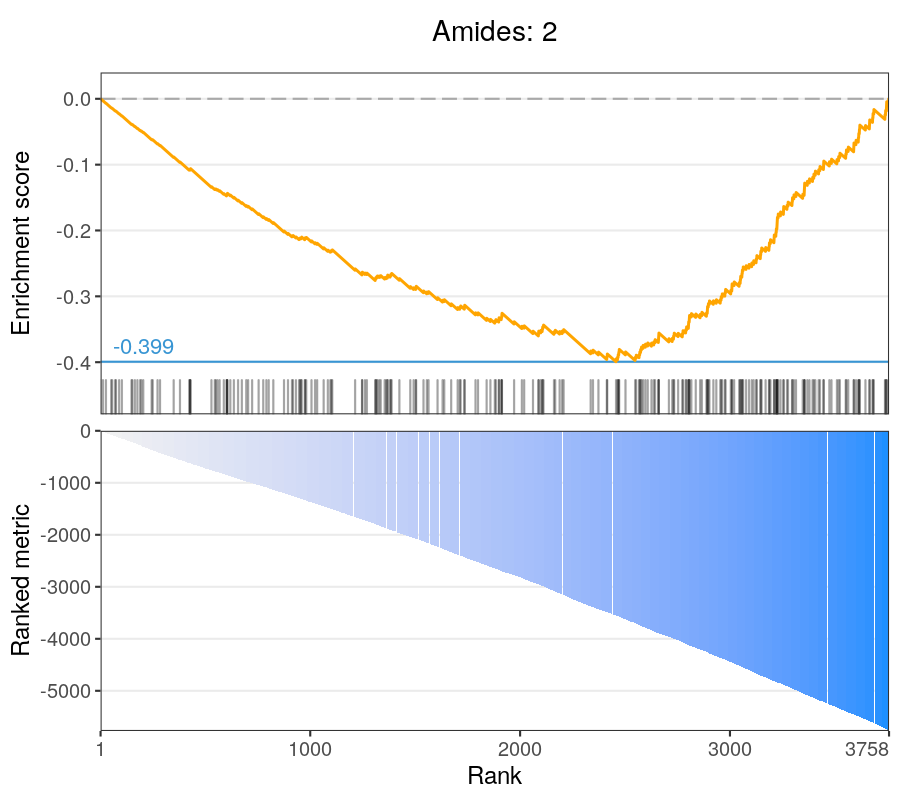
\includegraphics[width=\textwidth]{images/ctrap/molecular-descriptors-a}
		\caption{\footnotesize{Rings Closures: 6 to 14}}
	\end{subfigure}
	\begin{subfigure}[h]{0.32\textwidth}
		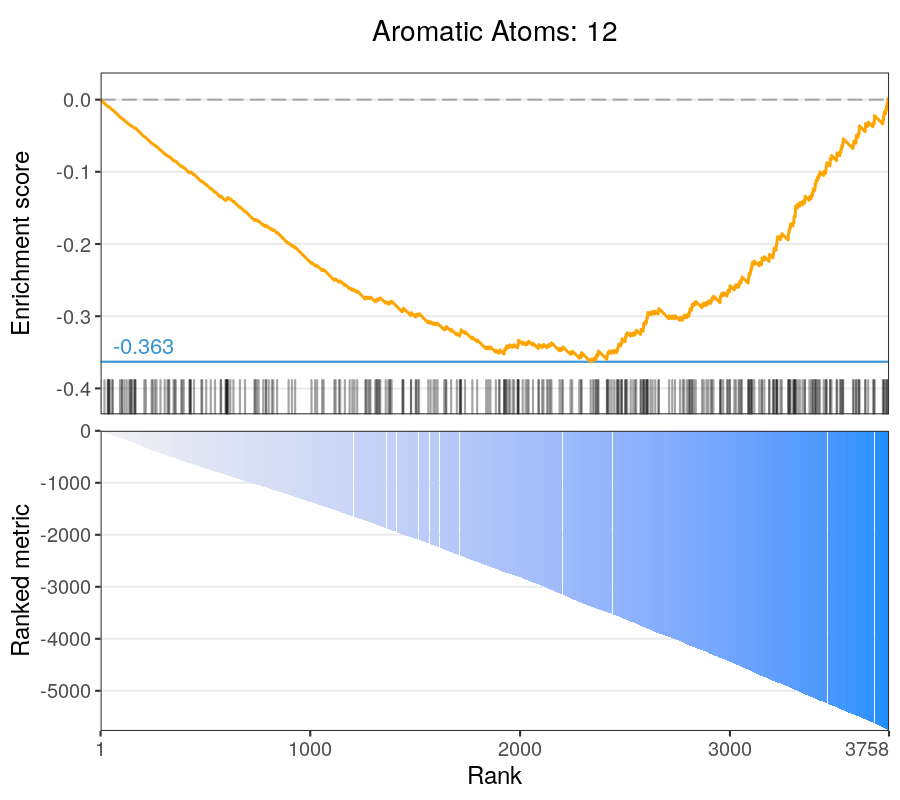
\includegraphics[width=\textwidth]{images/ctrap/molecular-descriptors-b}
		\caption{\footnotesize{Rings Closures: 0 to 1}}
	\end{subfigure}
	\begin{subfigure}[h]{0.32\textwidth}
		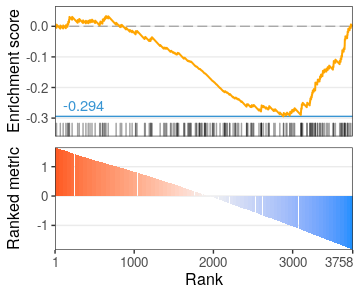
\includegraphics[width=\textwidth]{images/ctrap/molecular-descriptors-c}
		\caption{\footnotesize{Rings Closures: 2}}
	\end{subfigure}
	\caption[Drug set enrichment analysis]{\textbf{Drug set enrichment analysis} on CMap compound perturbations ranked by similarity to \emph{EIF4G1} knockdown phenotype. GSEA plots displayed for select molecular descriptors with adjusted p-value $< 0.05$. The rank metric is the scaled and centred additive inverse of the rank product's rank.}
	\label{fig:ctrap-descriptors}
\end{figure}

\subsection{Time and memory optimisation}
\label{subsec:ctrap-optim}

cTRAP allows comparing user-provided differential expression results against the CMap perturbation z-scores that are contained in a 21GB GCTx file. The GCTX format stores annotated, high-dimensional data matrices and is based on the HDF5 format for efficient indexing and loading of subsets of the whole data \cite{enache:2018wq}. Instead of loading the whole GCTx file into memory, cTRAP 1.4 and newer versions minimise peak RAM usage by loading and processing user-selected subsets of perturbation z-scores (e.g., only compound perturbations) in chunks of 1 GiB (default).

Although processing data by chunks helped reducing the memory footprint of cTRAP, we later refactored the code of the comparisons in cTRAP 1.10, a milestone that included multiple improvements to speed and memory:

\begin{itemize}
	\item Faster WTCS calculation by improving code efficiency.
	\item Slightly improved runtime by avoiding redundant loading of data chunks. This change was also required to enable multi-thread support in systems that implement process forking (e.g., Linux and macOS, but not Windows).
	\item Optional argument to set a custom size for data chunks (1 GiB by default).
	\item As the NCI-60 gene expression and drug sensitivity correlation matrix is also large (3.3GB), we saved that matrix as a HDF5 file that is then loaded and processed by cTRAP in chunks of 1 GiB (by default), minimising peak RAM usage when predicting targeting drugs based on the NCI-60 data.
\end{itemize}

We benchmarked time and memory when ranking CMap perturbations based on Spearman's correlation, Pearson's correlation and WTCS using a development version of cTRAP 1.10 (commit \link{https://github.com/nuno-agostinho/cTRAP/commit/296f9b2}{296f9b2}) and using as query the t-statistics for differential expression of \emph{EIF4G1} knockdown in HepG2 cells from ENCODE. The number of CMap compound perturbations (241 258) is much higher than those of the knockdown (48 862) and over-expression (24 627) perturbations and this is expected to reflect on time and memory for data processing.

When ranking CMap compound perturbations in cTRAP 1.8 and 1.10, the runtime was decreased from 95 to 53 minutes when loading the whole data and from 77 to 28 minutes when loading by chunks (\autoref{fig:cmap-ranking-time}). For each chunk, we parallelised the calculations performed per perturbation and this can help to speed up runtime, with 4 threads, from 28 to 12 minutes. However, the usage of 8 threads is not recommended as the runtime is similar to using 4 threads while consuming more resources.

\begin{figure}[!ht]
  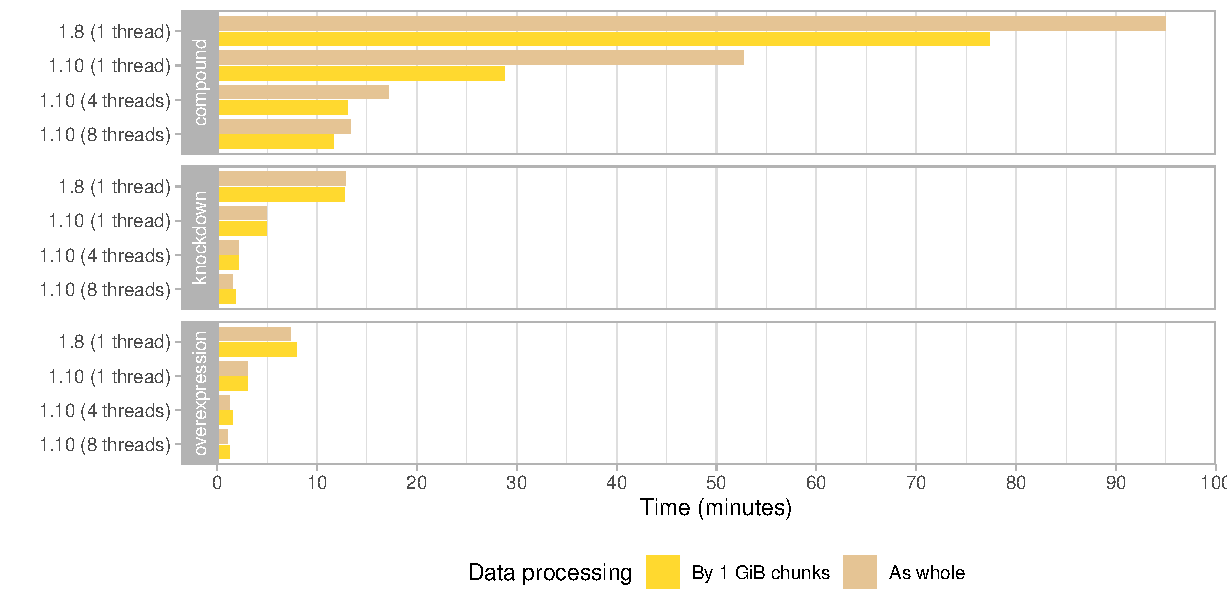
\includegraphics[width=\textwidth]{images/ctrap/ranking-time}
  \centering
  \caption[Time benchmark of CMap perturbation ranking]{\textbf{Time benchmark of CMap perturbation ranking.} Times were measured for cTRAP 1.8 (1 thread only) and 1.10 (1, 4 and 8 threads) for over-expression, knockdown and compound perturbations whose data was loaded by 1 GiB chunks or as whole.}
  \label{fig:cmap-ranking-time}
\end{figure}

Benchmarked memory was annotated based on the different internal steps performed by cTRAP (\autoref{fig:cmap-ranking-memory}). When ranking against the CMap compound perturbations, loading and processing their z-scores at once requires 59.7 GiB, compared to 5.4 GiB when loading and processing 1 GiB chunks. The differences were not as stark when using the knockdown and over-expression perturbations, but were still crucial to allow the possibility of running cTRAP in a common laptop with 8 GiB of RAM. % Although memory profiling expectedly slows down runtime, we can also see in the memory benchmark that loading data by chunks can have a big impact on elapsed time of a run when comparing compound perturbations.

\begin{figure}[!ht]
  \vspace{-\intextsep}
  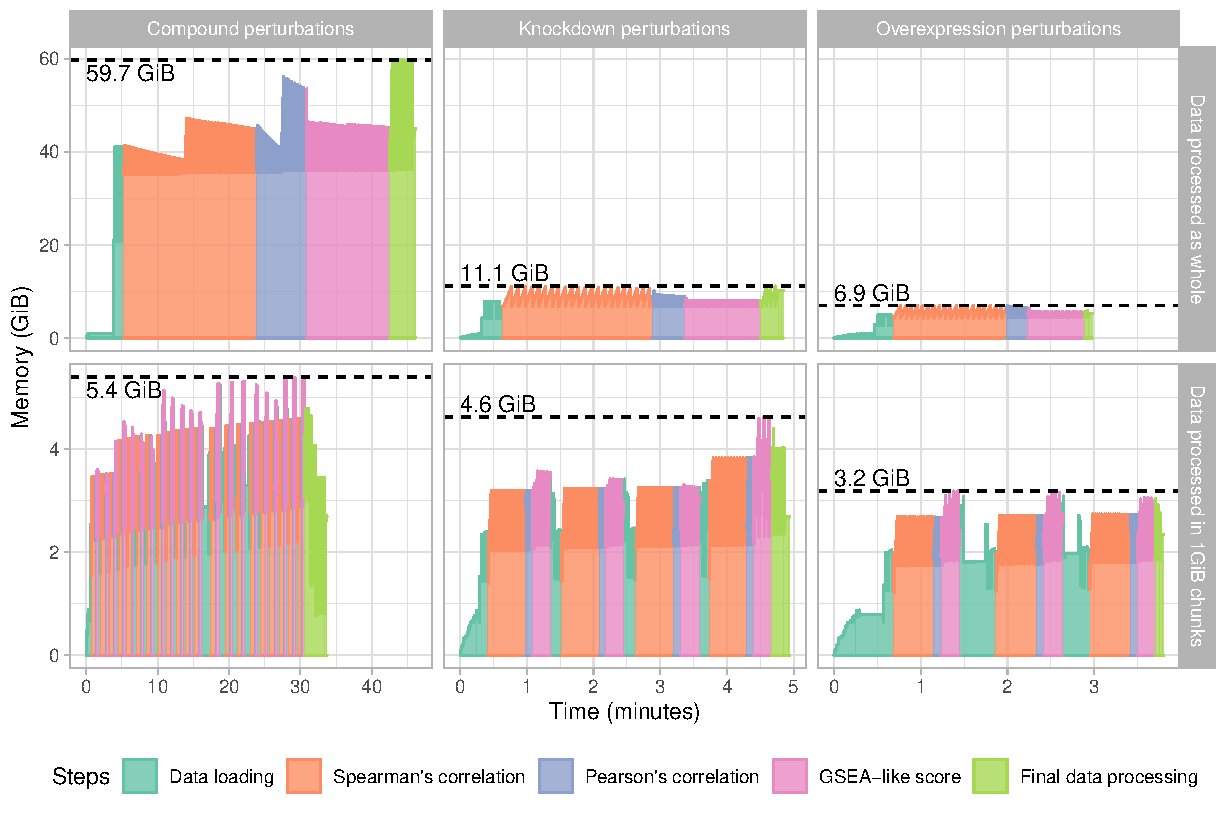
\includegraphics[width=\textwidth]{images/ctrap/ranking-memory}
  \centering
  \vspace{-\intextsep}
  \caption[Memory benchmark of CMap perturbation ranking]{\textbf{Memory benchmark of CMap perturbation ranking,} annotated using the different steps performed by cTRAP. Memory was benchmarked when ranking compound, knockdown and overexpression perturbations against differential expression results. The maximum memory used for each condition is labelled.}
  \label{fig:cmap-ranking-memory}
\end{figure}

\subsection{Graphical interface}

To assist users that may prefer graphical interfaces, most cTRAP functionality is exposed via 5 modular and independent Shiny-based functions (\autoref{fig:ctrap-ui-functions}):

\begin{itemize}
	\item \texttt{launchDiffExprLoader()} to load differential expression data. Returns a differential expression object that can be used in cTRAP analyses.
	\item \texttt{launchCMapDataLoader()} to explore and load CMap data by type of perturbation, cell types, time points and dosages. Returns filtered CMap data based on the user's selection.
	\item \texttt{launchMetadataViewer()} to check metadata of given cTRAP objects.
	\item \texttt{launchResultPlotter()} to view and plot cTRAP results given as input.
	\item \texttt{launchDrugSetEnrichmentAnalyser()} to analyse drug set enrichment and visualize respective results.
\end{itemize}

\begin{figure}[!ht]
	\centering
	\begin{subfigure}[h]{0.3\textwidth}
		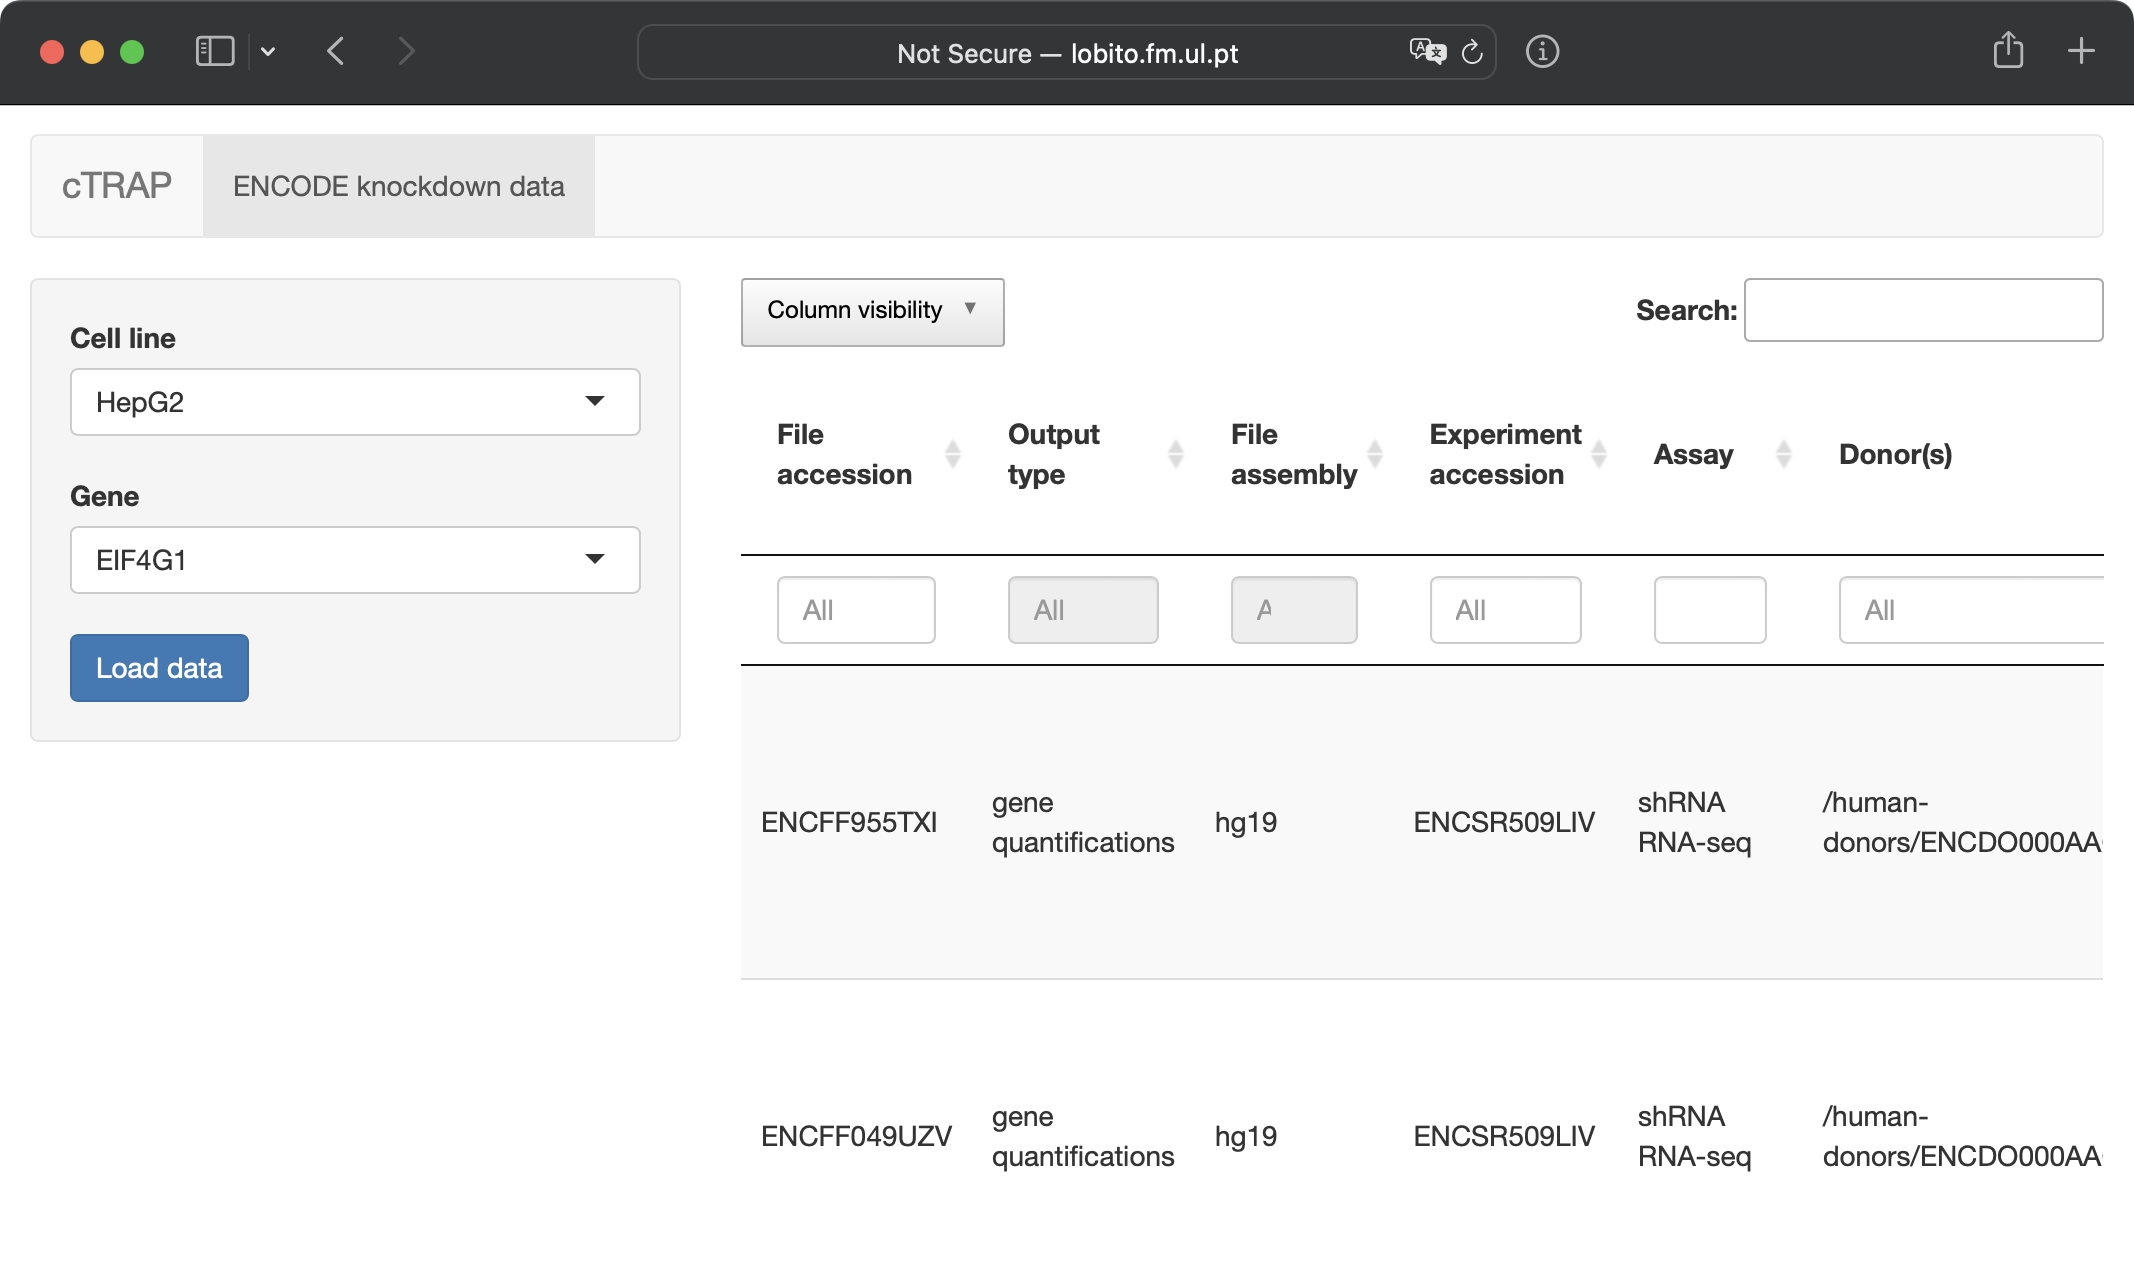
\includegraphics[width=\textwidth]{images/ctrap/ui/launchDiffExprLoader}
		\caption{\footnotesize{\texttt{launchDiffExprLoader}}}
	\end{subfigure}
	\begin{subfigure}[h]{0.3\textwidth}
		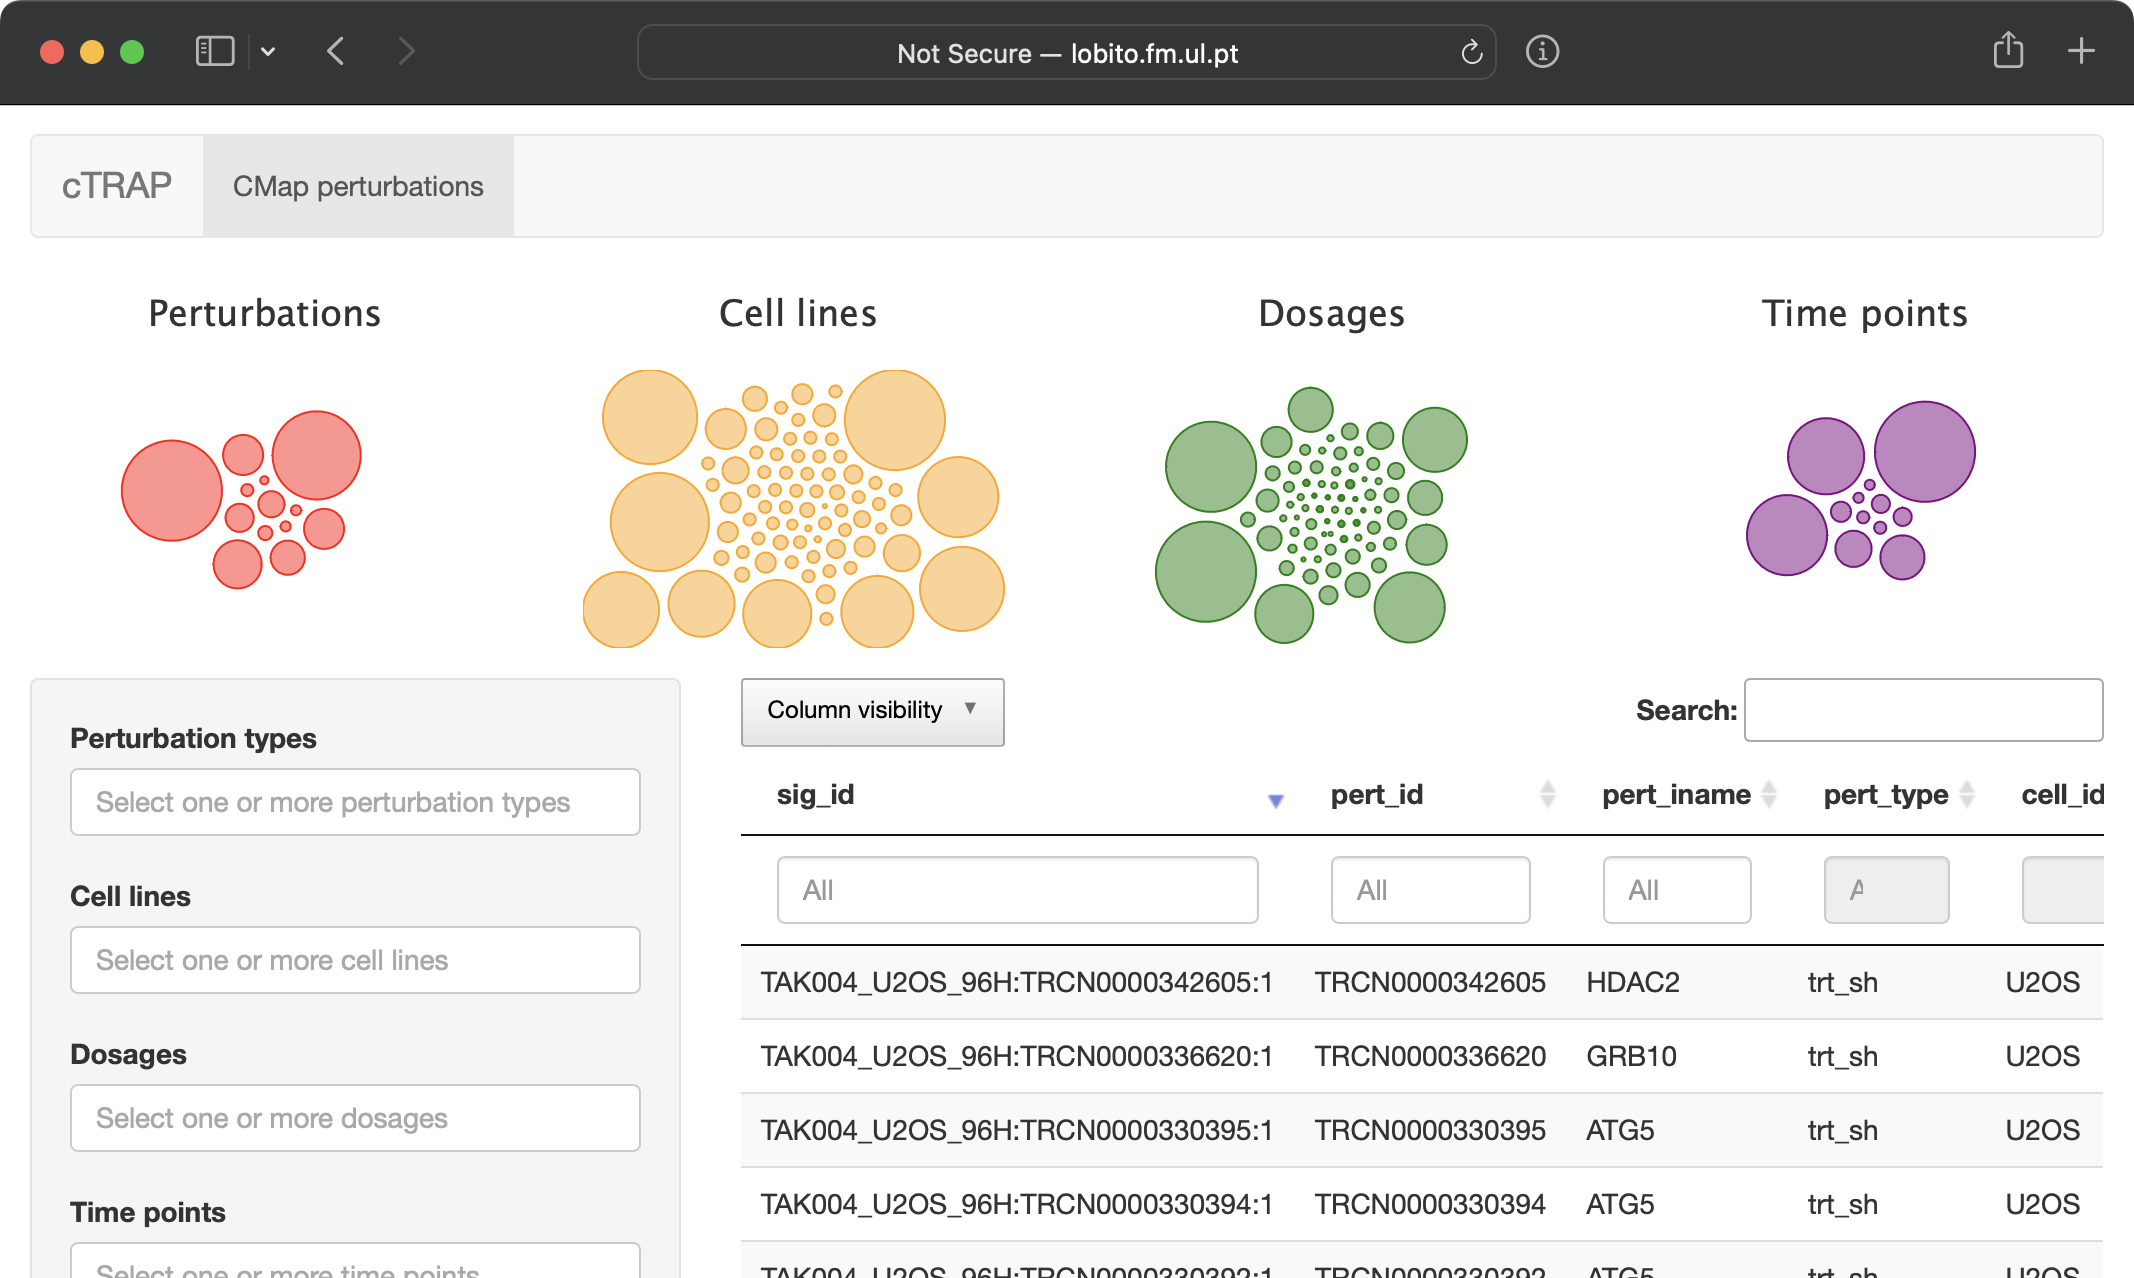
\includegraphics[width=\textwidth]{images/ctrap/ui/launchCMapDataLoader}
		\caption{\footnotesize{\texttt{launchCMapDataLoader}}}
	\end{subfigure}
	\begin{subfigure}[h]{0.3\textwidth}
		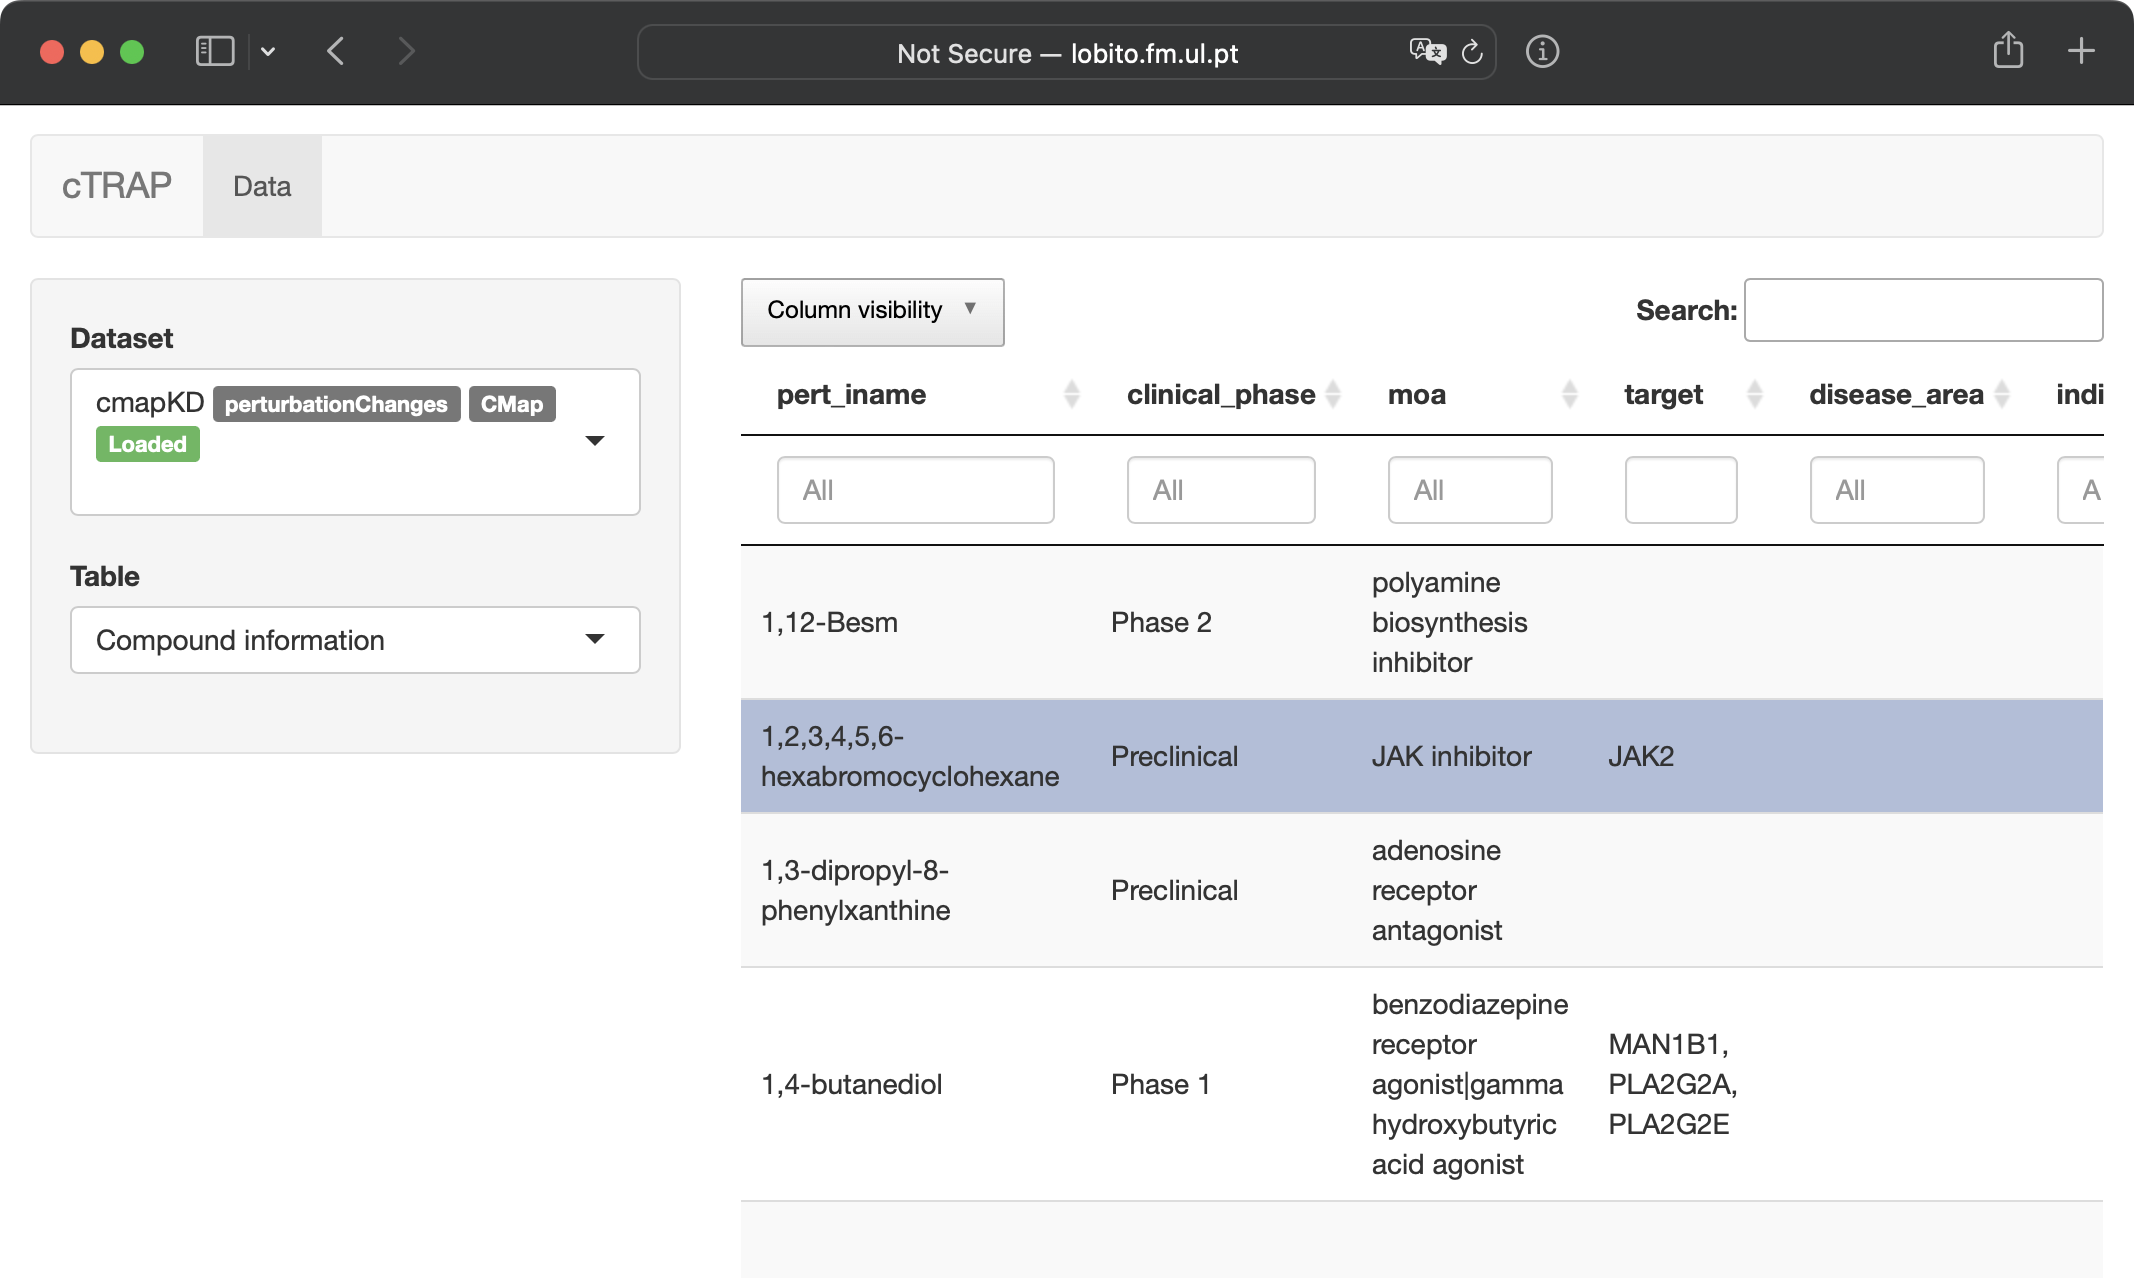
\includegraphics[width=\textwidth]{images/ctrap/ui/launchMetadataViewer}
		\caption{\footnotesize{\texttt{launchMetadataViewer}}}
	\end{subfigure}
	\begin{subfigure}[h]{0.45\textwidth}
		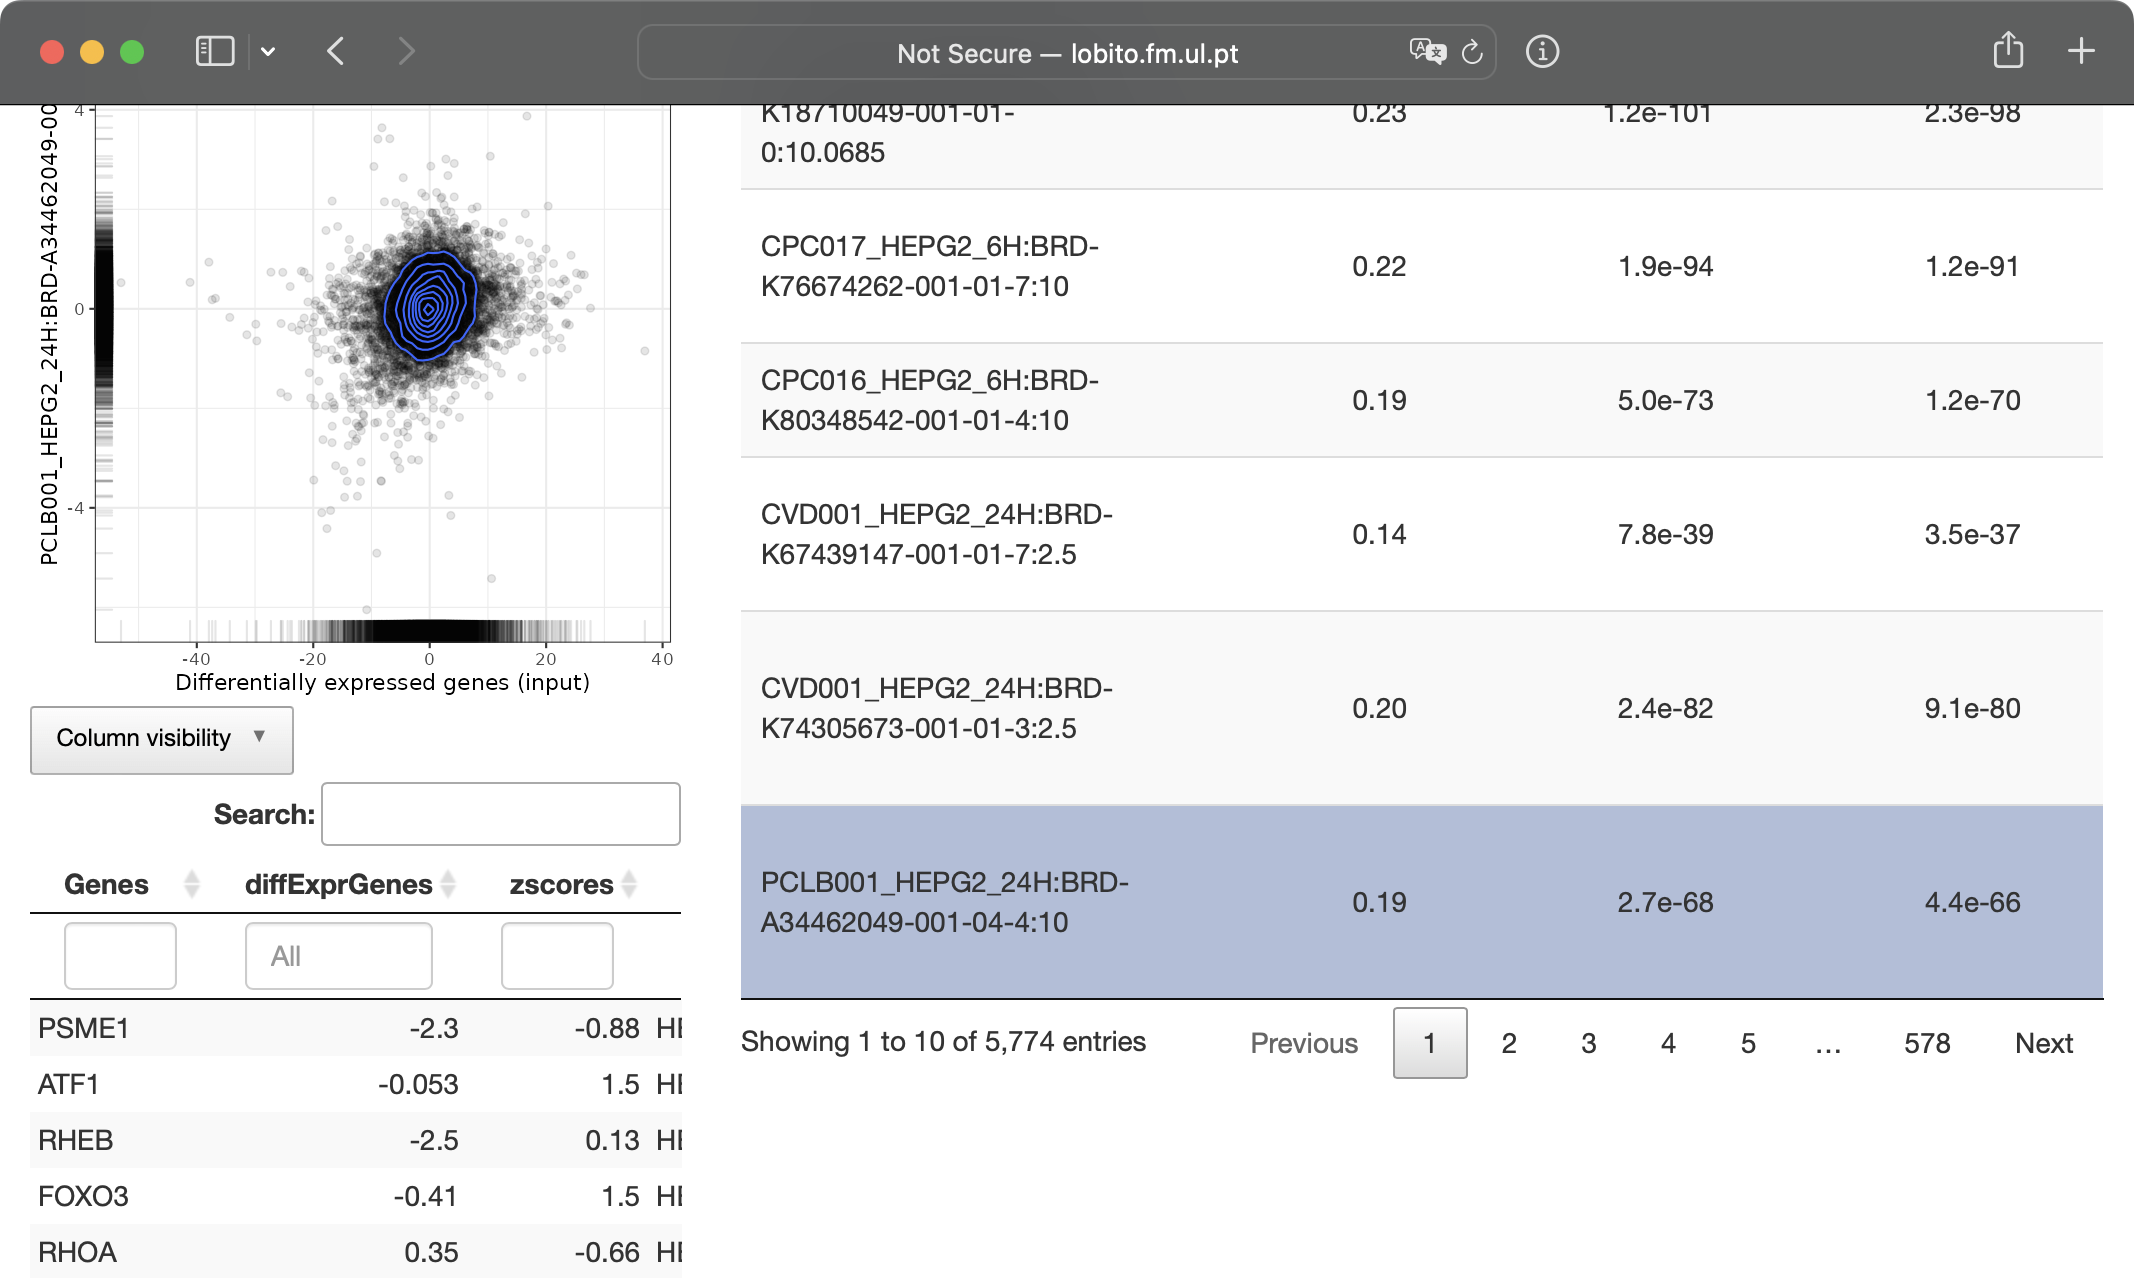
\includegraphics[width=\textwidth]{images/ctrap/ui/launchResultPlotter}
		\caption{\footnotesize{\texttt{launchResultPlotter}}}
	\end{subfigure}
	\begin{subfigure}[h]{0.45\textwidth}
		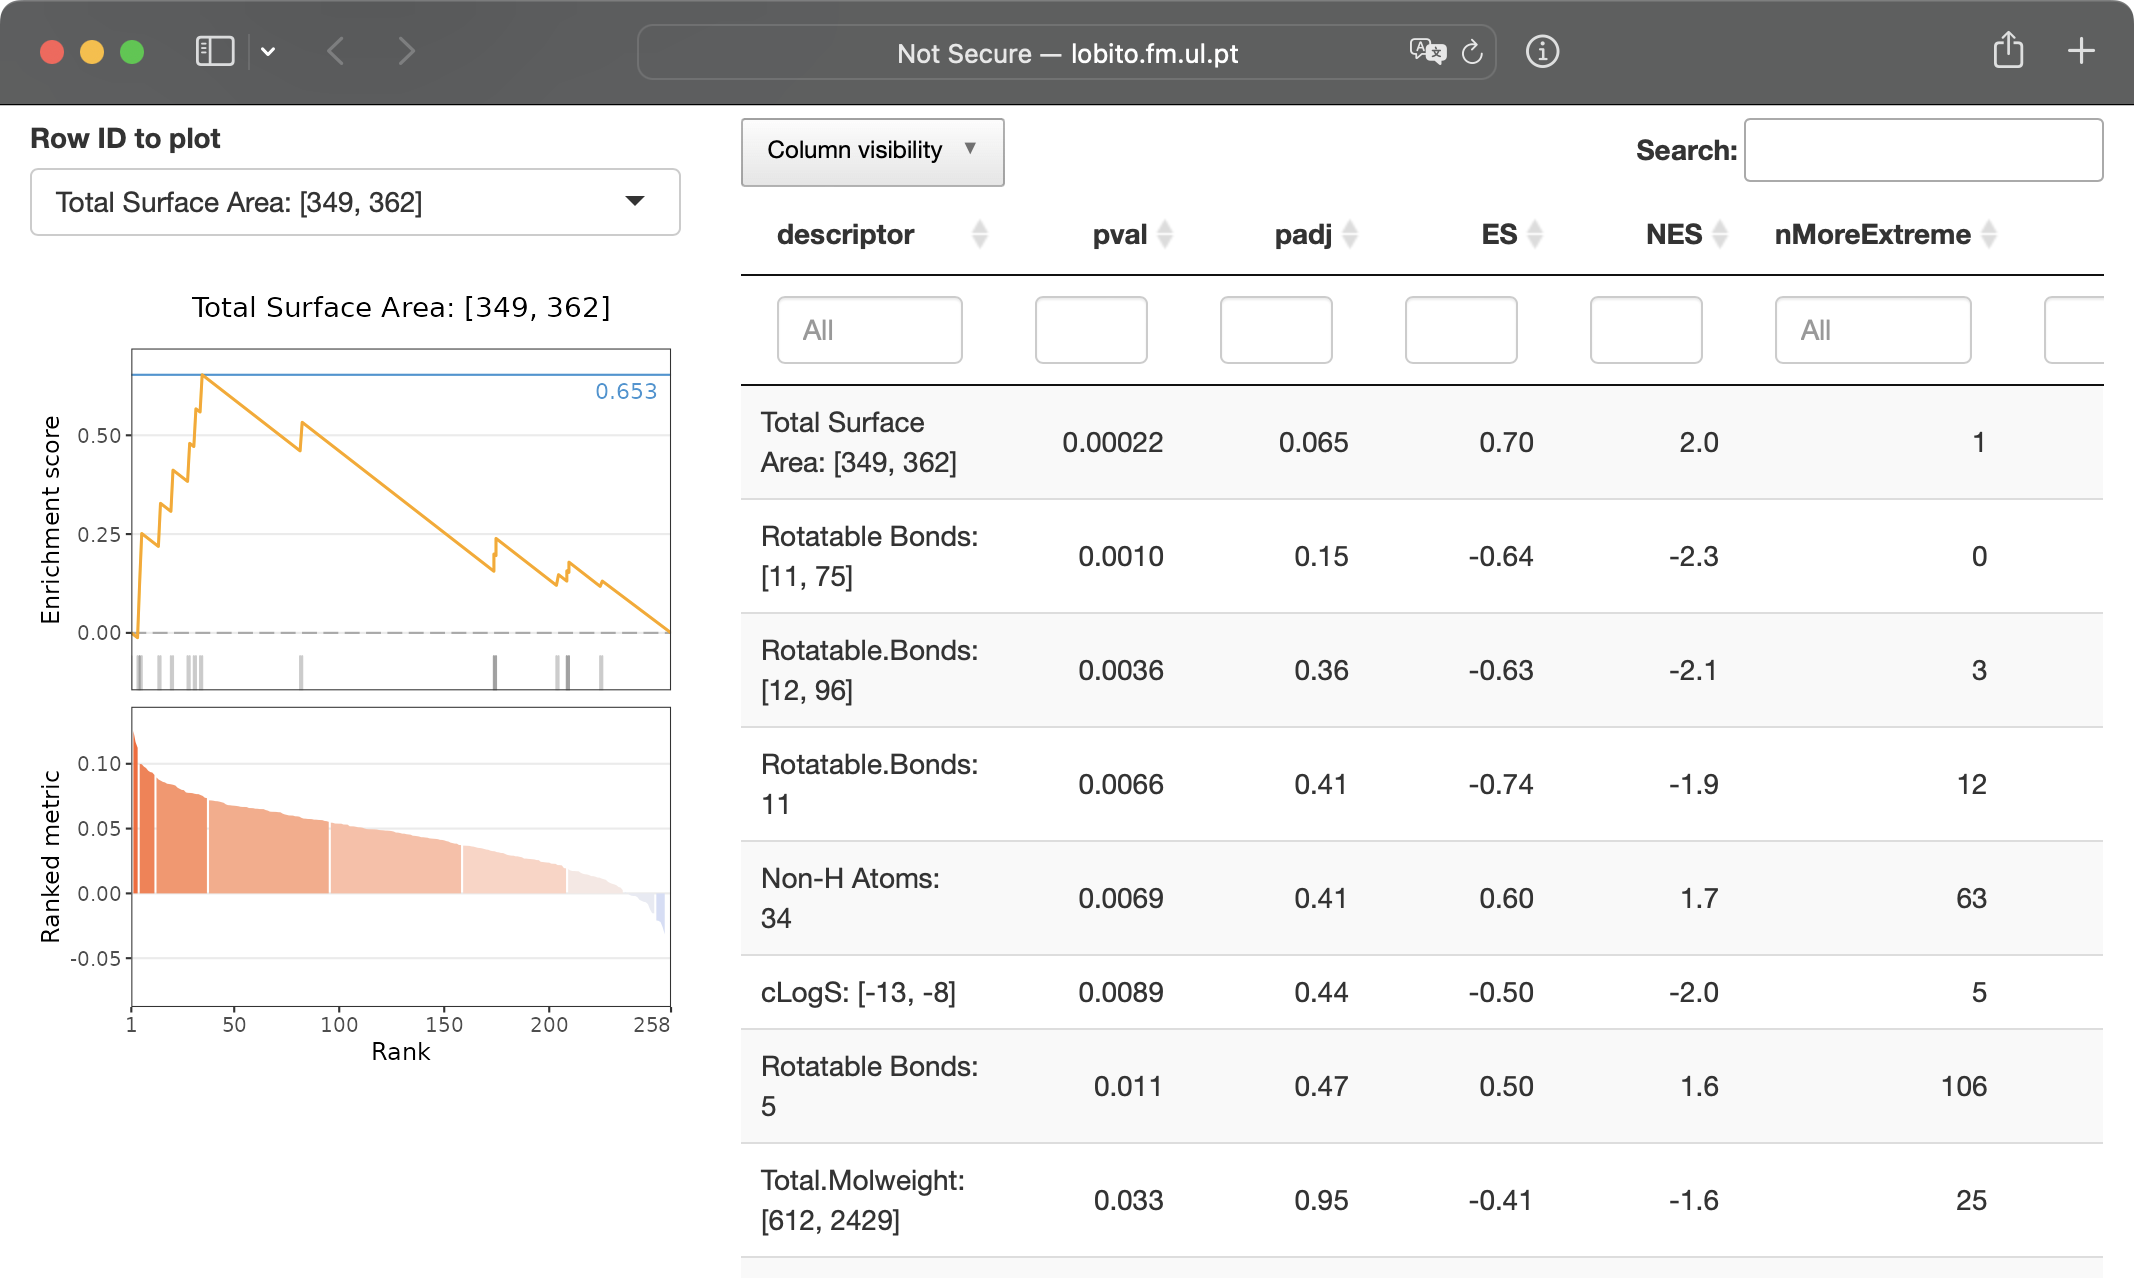
\includegraphics[width=\textwidth]{images/ctrap/ui/launchDrugSetEnrichmentAnalyser}
		\caption{\footnotesize{\texttt{launchDrugSetEnrichmentAnalyser}}}
	\end{subfigure}
	\caption[cTRAP graphical interface functions]{\textbf{Screenshots of the modular cTRAP graphical interface functions}.}
	\label{fig:ctrap-ui-functions}
\end{figure}

Like usual R functions, these graphical interface functions accept input arguments and may return output, allowing to intertwine them with R code (\shortref{lst:cTRAP-graphical}). Therefore, users can interactively prepare and explore data before running long-running tasks in the command-line, avoiding the need to have Shiny working while the tasks run (which may also slow down those tasks) and allowing to parallelise them.

\begin{lstlisting}[caption=Calling cTRAP's graphical interface functions in an R script.,label={lst:cTRAP-graphical},language=R,morekeywords={include, launchDiffExprLoader},keywordstyle=\bfseries]
library(cTRAP)

# Launch differential expression loading interface to select knockdown
# data from ENCODE (pre-filtered for HepG2 cell line and EIF4G1 gene)
diffExpr <- launchDiffExprLoader(cellLine="HepG2", gene="EIF4G1")
# After filter selection, launchDiffExprLoader() does the following:
# 1. Download ENCODE's HepG2 data for EIF4G1 knockdown and controls
# 2. Perform DGE between EIF4G1 knockdown vs. control
# 3. Return resulting t-statistics by gene

# Load CMap knockdown data in HepG2
cmapKD <- launchCMapDataLoader(
    cellLine="HepG2",
    perturbationType="Consensus signature from shRNAs targeting the same gene")
# Load CMap compound data in HepG2
cmapCompounds <- launchCMapDataLoader(cellLine="HepG2",
                                      perturbationType="Compound")
# Load all CMap data in HepG2
cmapPerts <- launchCMapDataLoader(cellLine="HepG2")

# View metadata of all resulting CMap data objects
launchMetadataViewer(cmapKD, cmapCompounds, cmapPerts)

# Rank similar perturbations -----------------------------------------
compareKD        <- rankSimilarPerturbations(diffExpr, cmapKD)
compareCompounds <- rankSimilarPerturbations(diffExpr, cmapCompounds)
comparePerts     <- rankSimilarPerturbations(diffExpr, cmapPerts)

launchResultPlotter(compareCompounds, compareKD, comparePerts)

# Predict targeting drugs --------------------------------------------
listExpressionDrugSensitivityAssociation()
assocMatrix <- listExpressionDrugSensitivityAssociation()[[1]]
assoc       <- loadExpressionDrugSensitivityAssociation(assocMatrix)
predicted   <- predictTargetingDrugs(diffExpr, assoc)
launchResultPlotter(predicted)

# Plot targeting drugs vs similar perturbations ----------------------
launchResultPlotter(predicted, compareCompounds)

# Analyse drug set enrichment ----------------------------------------
descriptors <- loadDrugDescriptors("NCI60", "3D")
drugSets    <- prepareDrugSets(descriptors)
launchDrugSetEnrichmentAnalyser(drugSets, compareCompounds)
launchDrugSetEnrichmentAnalyser(drugSets, predicted)
\end{lstlisting}

cTRAP also provides a Shiny-based global visual interface that encompasses all graphical interface modules into one web app by running function \texttt{cTRAP()}, the basis for its online version\footnote{More information in \fullref{chap:app-server}.}. However, that implementation for a single interface would mean that each cTRAP session needed to be live and consume useful resources during the long-running cTRAP analyses, which does not properly scale in a web server with multiple users requiring heavy memory resources simultaneously. To circumvent this issue, long-running tasks can be optionally managed via job queues running in the background. In order for users to redeem their results once they finish calculating, we also implemented storage and retrieval of user session data in cTRAP.

\subsubsection{User session data}
\label{sec:ctrap-web}

Session data are saved in folders named after a random alphanumeric string (token) that uniquely identifies each session and can be downloaded as an RDS file -- a list containing data for all datasets from the user session. Users can load these RDS files in any R session and in local instances of cTRAP. Downloading user sessions is encouraged because cTRAP session folders are removed from our server if not accessed in the last 30 days based on the access timestamp to optimise resources and scalability with multiple users\footnote{In Linux, the access timestamp (\texttt{atime} attribute) for a directory indicates the last time a file within was read/written or its contents were listed.}.

\begin{wrapfigure}{r}{.4\textwidth}
  \vspace{-2\intextsep}
  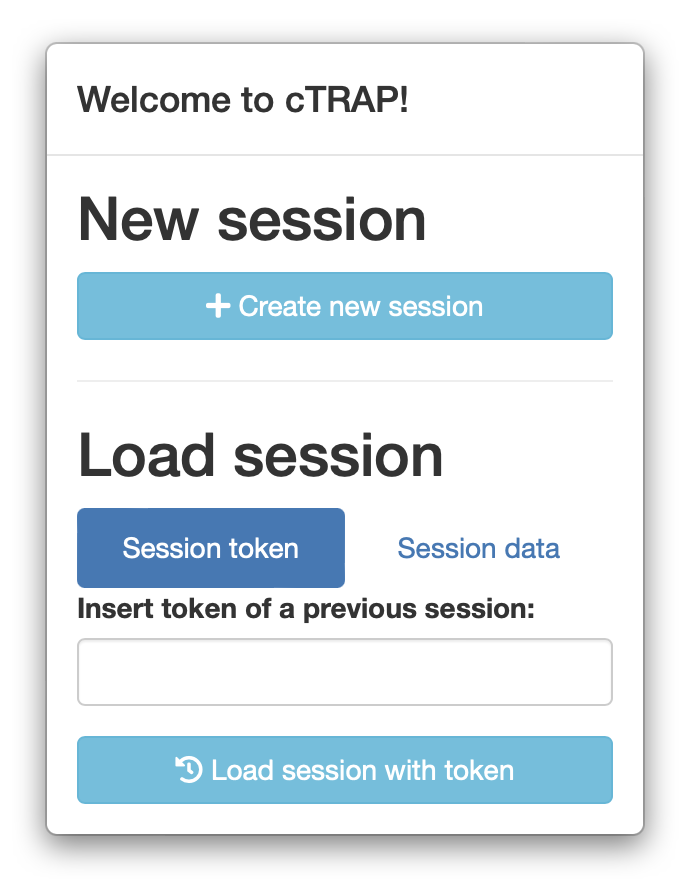
\includegraphics[width=\linewidth]{images/ctrap/welcome}
  \caption[Welcome screen modal]{\textbf{Welcome modal.}}
  \vspace{-1\intextsep}
  \label{fig:ctrap-welcome}
\end{wrapfigure}

cTRAP visitors are greeted with a welcome screen that allows them to create a new session or restore previous ones (\autoref{fig:ctrap-welcome}), a dialog that can be opened at any time from the session menu.

% TODO: mention other files in common across cTRAP?
When creating a new session, a unique token is created. As soon as session-specific data are loaded, a new folder is created in the working directory and named after the session token (\autoref{fig:user-session}). Any updates to the session data are automatically saved to the session folder. To avoid downloading commonly-used files (e.g., the 21GB CMap perturbations z-scores file), an appropriate folder stores data shared across sessions, thus avoiding downloading, storing and processing redundant data.

\begin{figure}[!ht]
  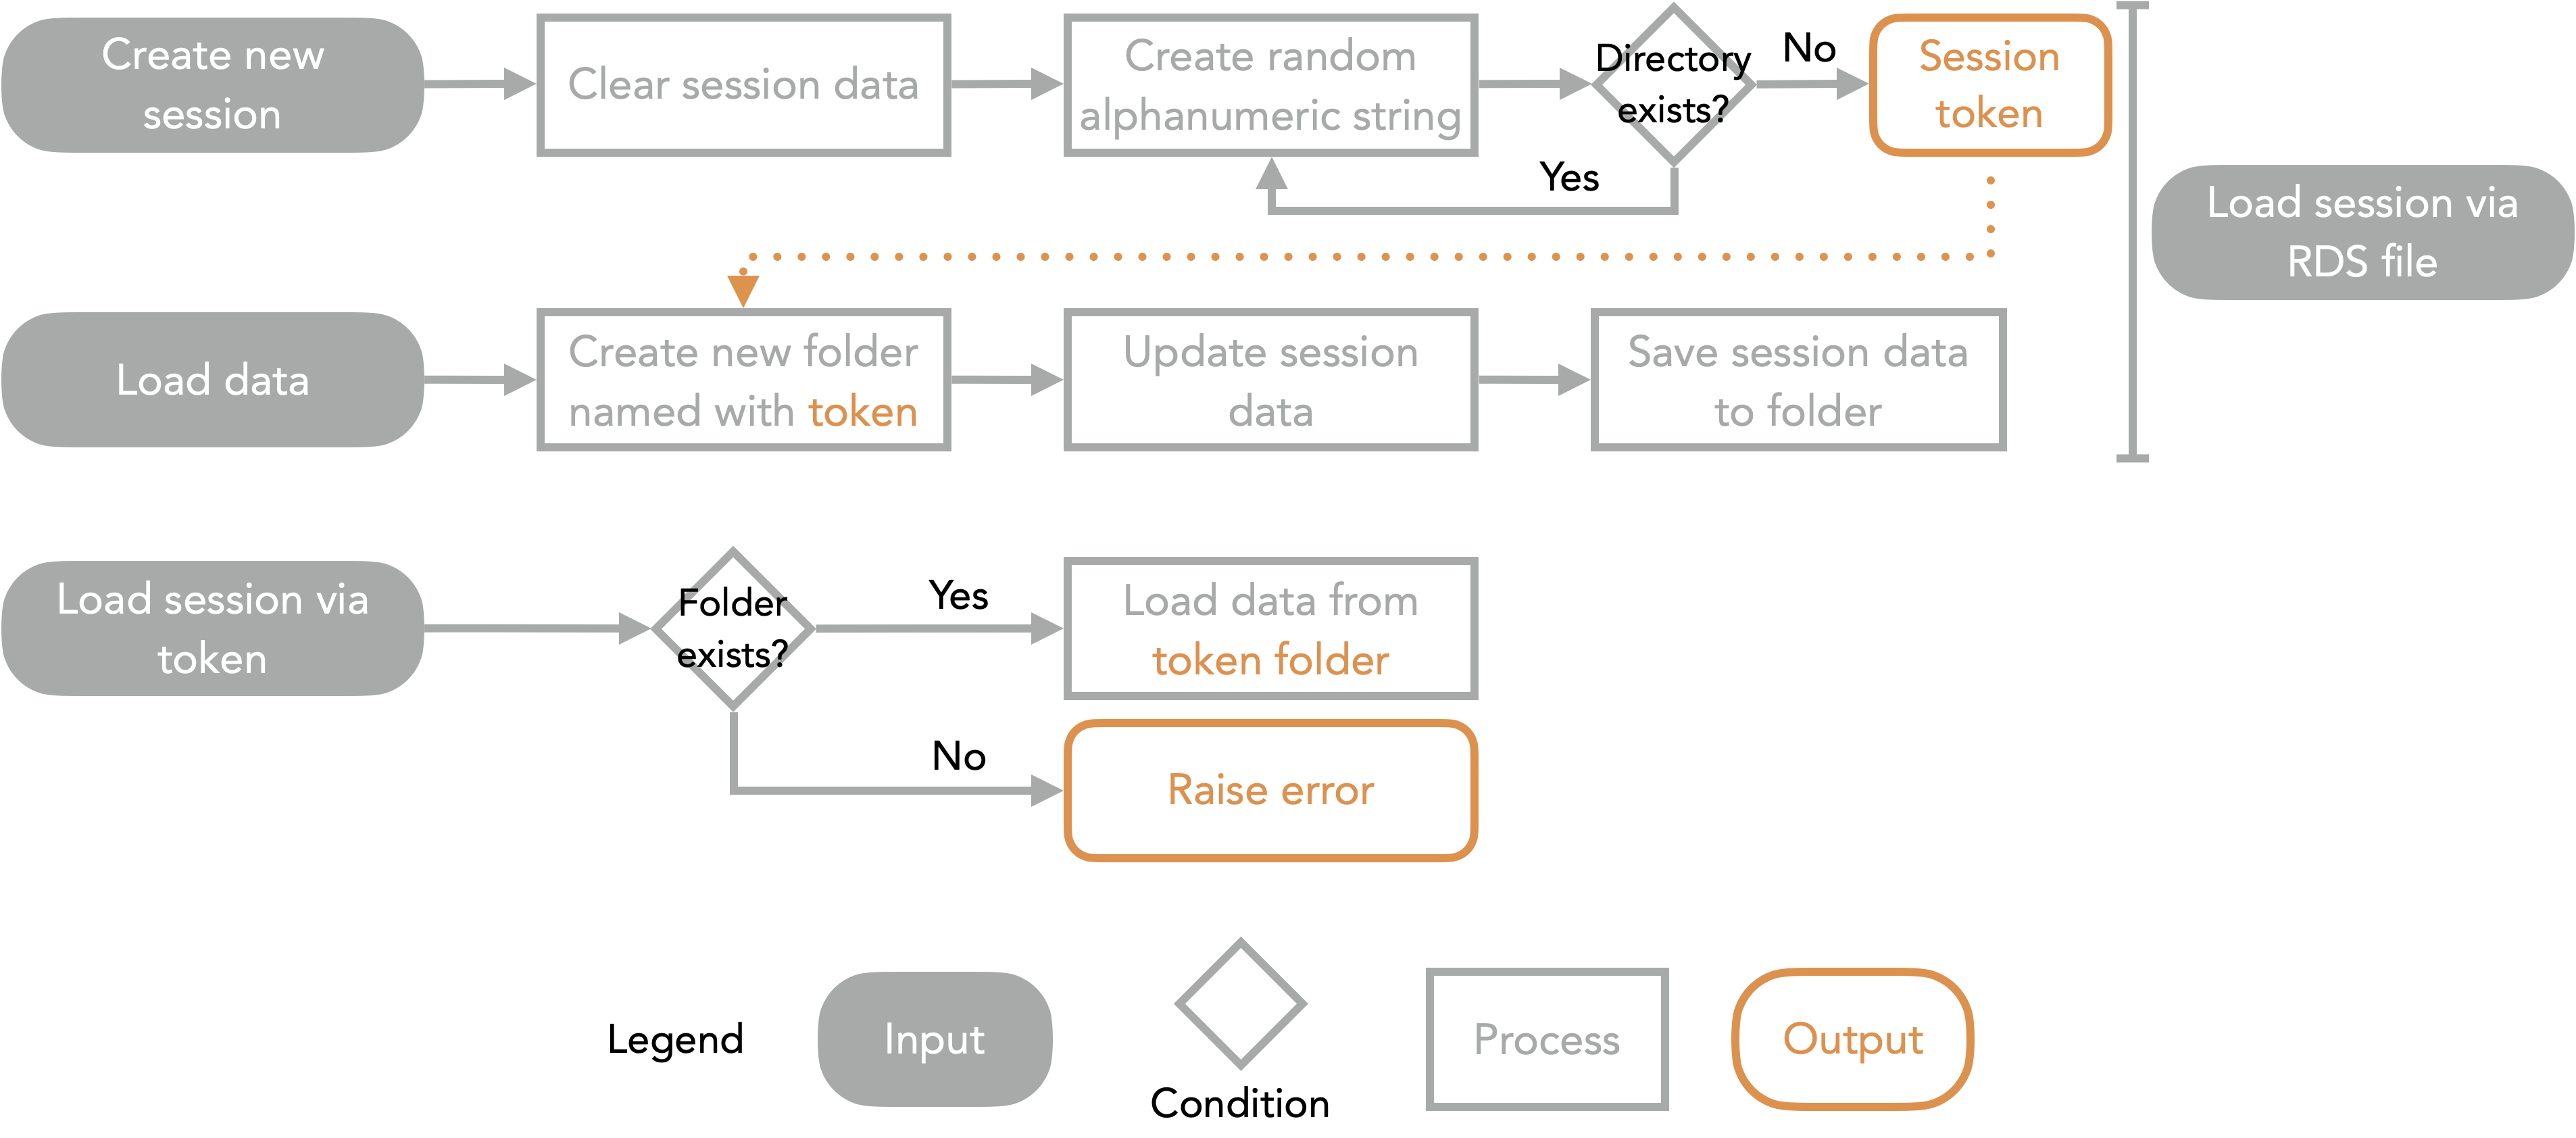
\includegraphics[width=\textwidth]{images/ctrap/user-session}
  \centering
  \caption[User session workflow]{\textbf{User session workflow.} cTRAP allows to create new sessions or load a previous one via a given token or RDS file. When loading session via a RDS file, a new cTRAP session is created before loading the data from RDS file. Sessions can also be loaded using a token if any folder with such token exists in cTRAP's working directory.}
  \label{fig:user-session}
\end{figure}

When restoring a session via a token, cTRAP loads the contents of the folder named after the token located in cTRAP working directory or warns the user if no such folder exists (\autoref{fig:user-session}). In case the user uploads the RDS file of a previous session, cTRAP will load its contents into a new session (\autoref{fig:user-session}).

\subsubsection{Background tasks}
\label{subsec:background-tasks}

When running a Shiny app, the user has to wait for all foreground tasks to finish before the app responds to user's commands. This issue can be mitigated by using R packages \texttt{promises}/\texttt{future} or by manually running another R process in the background. However, these solutions require the Shiny app to be active during the whole process, which can be especially egregious if the R session is consuming many computing resources, disallowing other apps or users to take advantage of those resources until the whole session is terminated.

Alternatively, we can use light-weight job schedulers to manage and run large tasks in the background, such as  \textbf{Celery}, a Python-based task queue manager that is complemented by \textbf{Flower}, a monitoring app that provides an HTTP API and graphical interface to manage Celery jobs.

Celery requires a \texttt{tasks.py} file detailing the tasks to run. As we intend to run R code submitted by cTRAP, we set up a Celery task that runs arbitrary R code by running the \texttt{Rscript} command via the \texttt{subprocess} Python module (\shortref{lst:tasks.py}).

\begin{lstlisting}[language=python,caption=An example \texttt{tasks.py} file to run R commands or Rscript files via Celery.,label={lst:tasks.py},morekeywords={import},keywordstyle=\bfseries]{tasks.py}
import os, time
from datetime import datetime
from subprocess import run, PIPE
# Celery configuration
from celery import Celery
os.environ.setdefault('C_FORCE_ROOT', 'true')
app = Celery(
    "tasks",
    broker=os.environ.get('CELERY_BROKER_URL', 'redis://redis'),
    backend=os.environ.get('CELERY_RESULT_BACKEND', 'redis://redis'))
app.conf.CELERY_WORKER_SEND_TASK_EVENTS = True

# Runs R command and returns output
#   - Use cat(), e.g., 'cat(2+2)', to capture output as a job result
#   - Errors will result in a task state of FAILURE
def execR(cmd):
    return run(cmd, check=True, stdout=PIPE, text=True).stdout

# Run a given R expression as a Celery job
@app.task
def R(cmd): return execR(["Rscript", "-e", cmd])

# Run a given Rscript file as a Celery job
@app.task
def Rscript(cmd): return execR(["Rscript", cmd])

if __name__ == "__main__": app.start()
\end{lstlisting}

Flower can assist job submission to Celery via HTTP methods, facilitating the communication between cTRAP and Celery. To assist using Flower in R, I created the R package \texttt{floweRy} (\alink{github.com/nuno-agostinho/floweRy}) that contains wrapper functions for most of its HTTP API functions. Internally, \texttt{floweRy} calls HTTP methods with the \texttt{httr} R package, creating dedicated commands that make it easier than using just plain \texttt{httr}, as briefly demonstrated in Listings \shorterref{lst:httr} and \shorterref{lst:floweRy}.

\noindent\begin{minipage}{.48\textwidth}
\begin{lstlisting}[caption=Job submission with \texttt{httr}.,language=R,label={lst:httr}]{httr}
library(httr)
flower <- function(...) paste0(
    "http://localhost:5555", ...)
# Run R command '3 + 4' in Celery
POST(flower("/api/task/apply/tasks.R")), body="3 + 4", encode="json")
# Get status of all Celery tasks
GET(flower("/api/tasks"))
\end{lstlisting}
\end{minipage}\hfill
\begin{minipage}{.48\textwidth}
\begin{lstlisting}[caption=Job submission with \texttt{floweRy}.,language=R,label={lst:floweRy}]{floweRy}
library(floweRy)
options(flowerURL=
    "http://localhost:5555")
# Run R command '3 + 4' in Celery
taskApply("tasks.R", "3 + 4")


# Get status of all Celery tasks
taskList()
\end{lstlisting}
\end{minipage}

cTRAP currently supports ranking similar CMap perturbation and predicting targeting drugs as background processes by submitting jobs to Celery with the exact R commands to run via the \texttt{Rscript} command \cite{r-core-team:2021wf}. Users can monitor the status of background tasks in their cTRAP session (\shortref{fig:job-progress})\footnote{Flower allows to monitor and manage Celery jobs, but its web interface is only accessible in the iMM network (via ethernet cable or VPN). More information in \fullref{sec:background-tasks}.}.

\begin{figure}[!ht]
  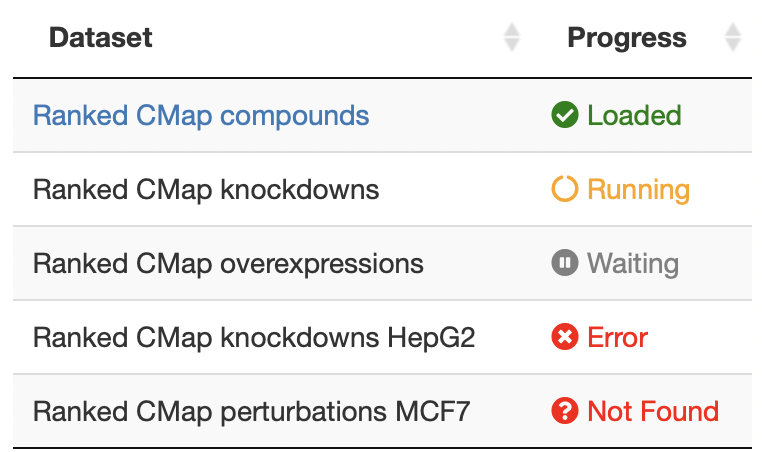
\includegraphics[width=.5\textwidth]{images/ctrap/job-progress}
  \centering
  \caption[Progress of Celery jobs in cTRAP]{\textbf{Progress of Celery jobs in cTRAP,} updated every 5 seconds. Job status can be: \textcolor{gray}{Waiting} in job queue to start, \textcolor{orange}{Running}, \textcolor{teal}{Loaded}, \textcolor{red}{Error} for unknown failures, and \textcolor{red}{Not Found} if the job results cannot be found (e.g., when re-uploading the same RDS file, the job results were already removed). When job results are loaded, the respective dataset name is a link to access them (in blue).}
  \label{fig:job-progress}
\end{figure}

All Celery jobs are saved as \emph{dummy} objects in cTRAP's user session data, containing the job identifier and metadata from expected results. When the background processes finish, their output is saved into the session folder. If the user is actively using that session in the cTRAP website, the data are automatically loaded -- replacing the previous \emph{dummy} objects -- and the user is informed of such via a notification in cTRAP (\shortref{fig:ctrap-celery}). Otherwise, the next time that session is loaded by the user (either via its token or an RDS file), the job for every \emph{dummy} object in the session data is returned if finished.

\begin{figure}[!htb]
  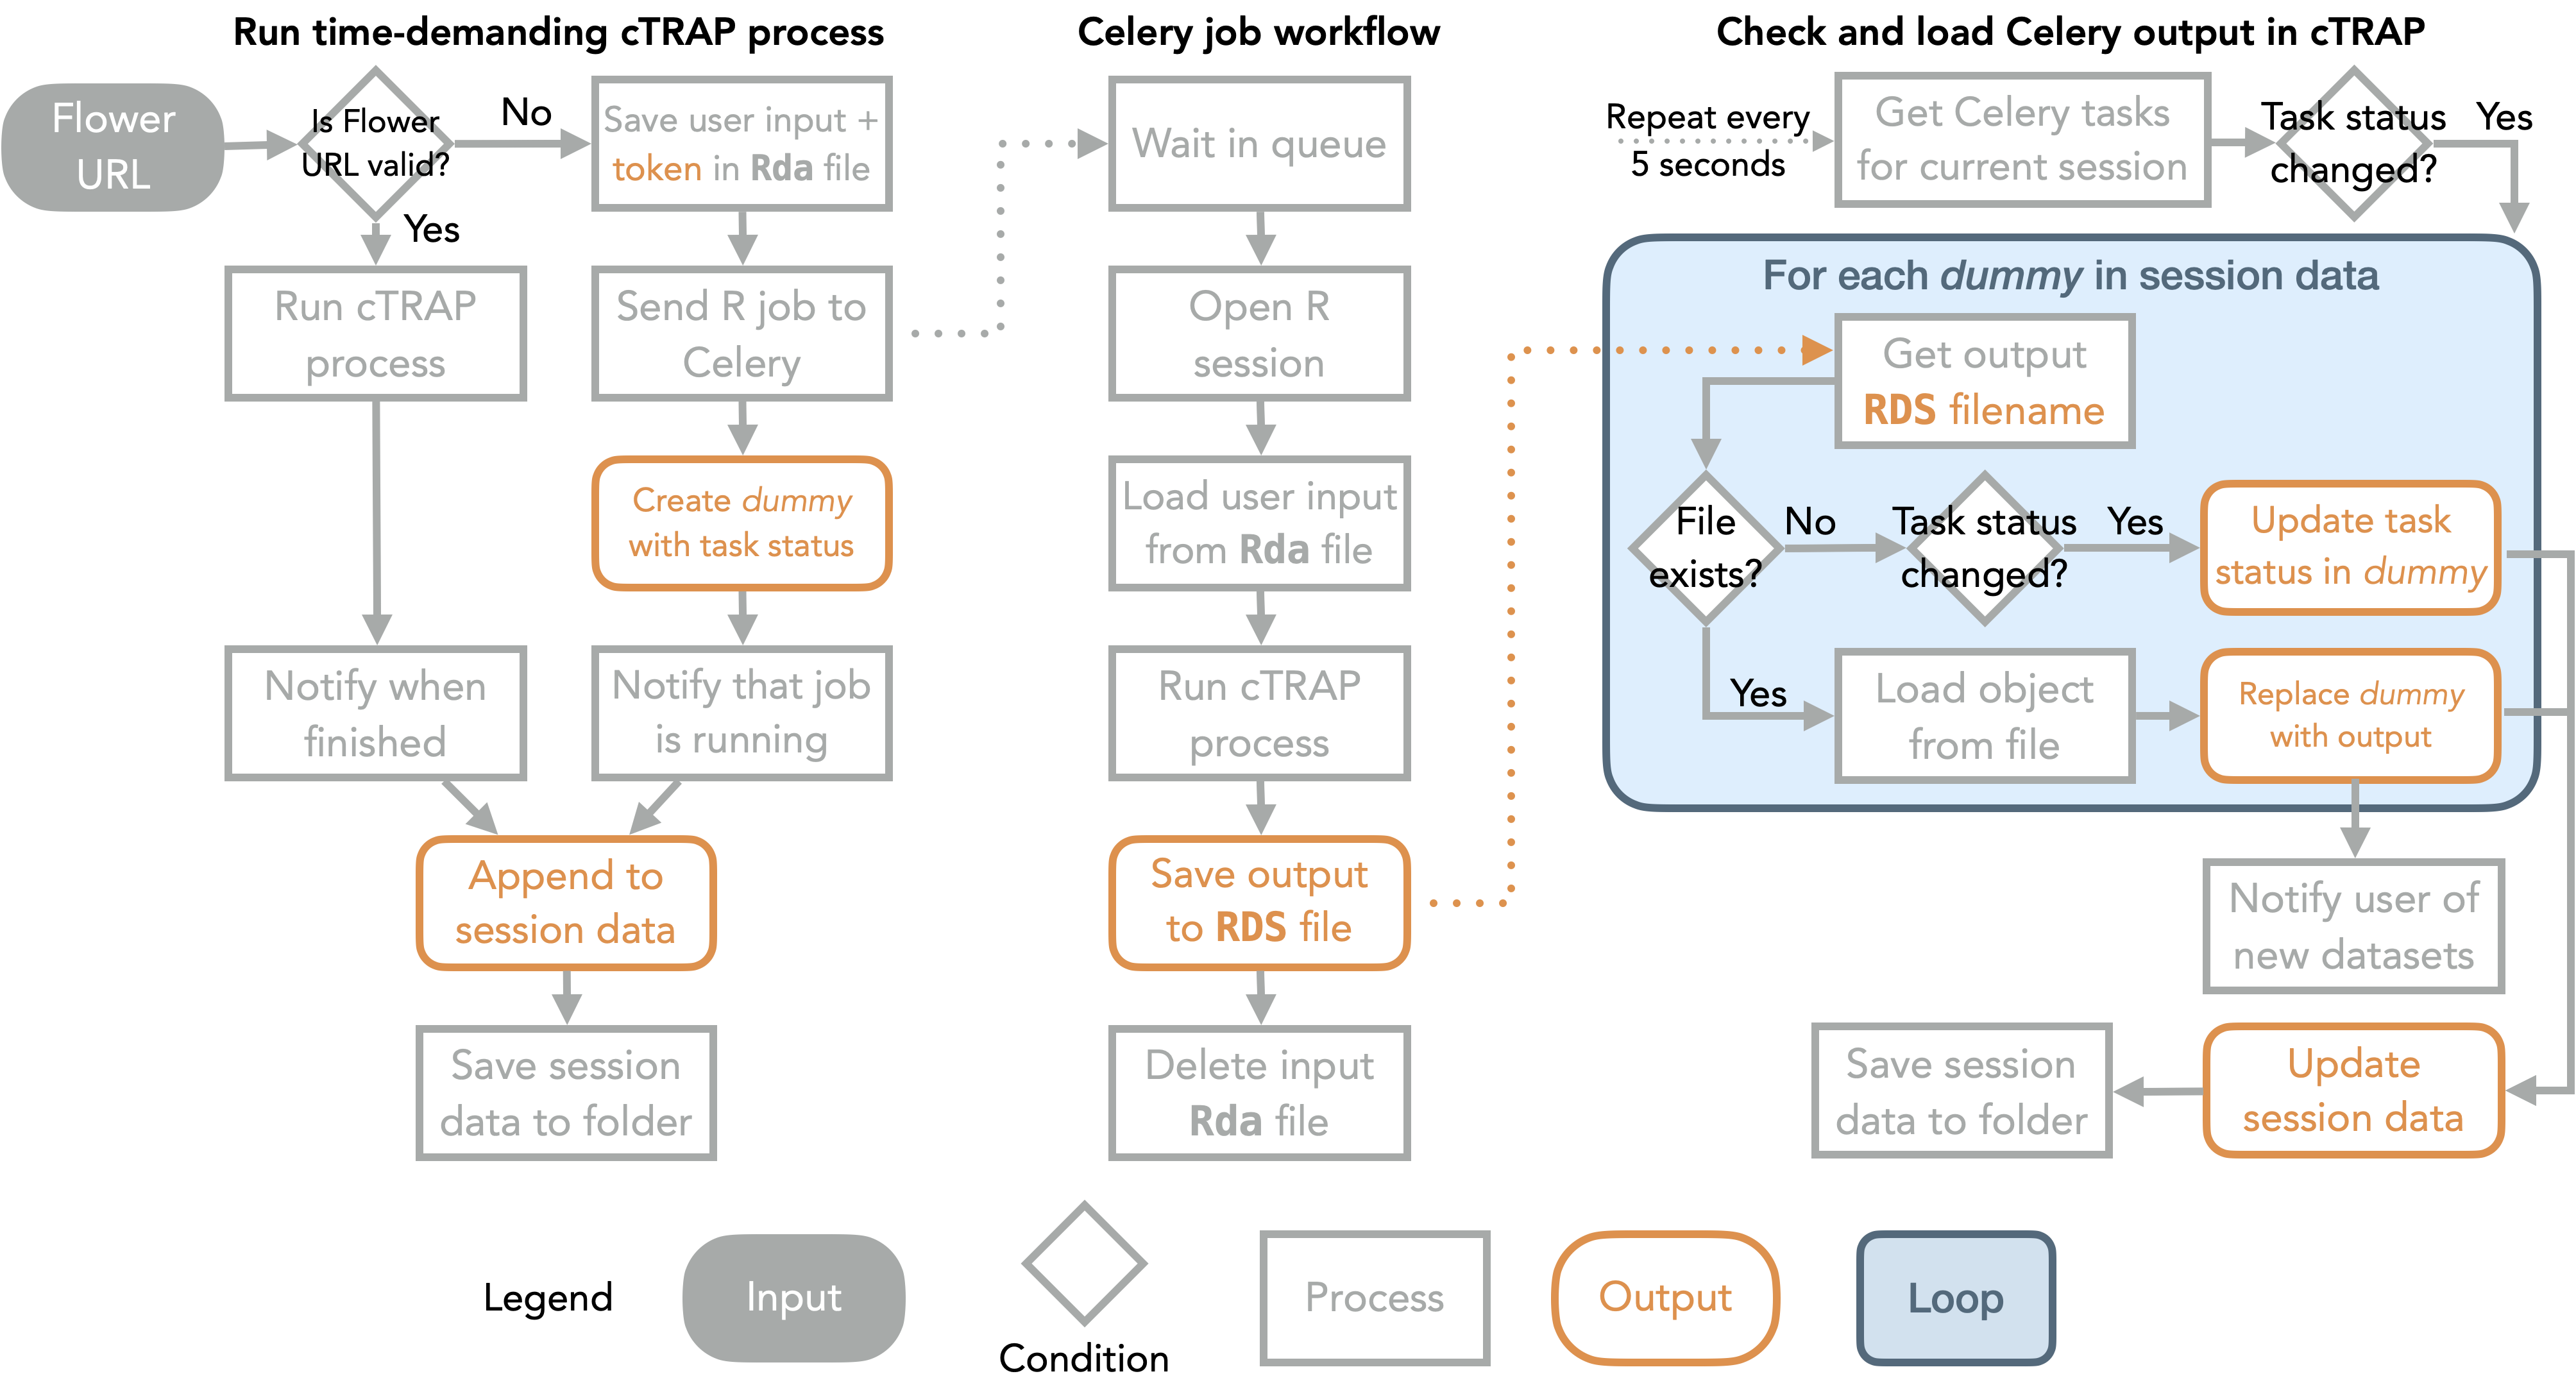
\includegraphics[width=\textwidth]{images/ctrap/celery-job}
  \centering
  \caption[cTRAP process running in Celery]{\textbf{cTRAP process running in Celery.} Time-demanding cTRAP processes can be run in the background using Celery/Flower. While running in Celery, the output of the cTRAP process is saved to the folder associated with the token of the user's session. When that specific session is active, all finished files are automatically loaded as part of the data session and the user is notified.}
  \label{fig:ctrap-celery}
\end{figure}

\section{Conclusion}

% what is your main finding (ANSWER)
% how are your findings with respect to the literature (POSITIONING)
% - RESULT: the actual results
% - CONTEXT: literature search
% - LINK: between my findings and what is known
% - INTERPRETATION: where you pinpoint, suggest, propose...
% what is your main contribution (CONTRIBUTION)
% what are the limitations (LIMITATIONS)
% what are the next steps (ENDING/FUTURE WORK)

The analysis of uncharacterised phenotypes may help understanding relevant biological insights and developing novel therapies by comparing changes in gene expression against a large reference database -- such as CMap -- containing differential expression data associated with known perturbagens \cite{subramanian:2017ul,hughes:2000ww}. The \alink{clue.io} website is a collection of web apps to explore CMap data and to compare user-provided differential expression results against those from genetic and pharmacological CMap perturbations \cite{subramanian:2017ul}. However, its shortcomings include limited queries with a maximum of 150 up-regulated and 150 down-regulated genes, poor automation with downstream analyses and lack of support to run with local computing resources.

We thus present cTRAP as a R package and web app to identify causal molecular perturbations from differential expression data, as well as pinpoint compounds that may promote or revert observed differences in gene expression. Besides the WTCS used by \alink{clue.io} that only considers the top 150 up- and top 150 down-regulated genes, cTRAP also allows to measure similarity based on Pearson's and Spearman's correlations, thus considering the expression of all common genes between datasets. Moreover, cTRAP allows to customise the number of up- and down-regulated genes in the set (by default, 150 like \alink{clue.io}). When performing multiple comparisons, cTRAP also returns the rank product's rank as a ranked summary of selected comparison methods.

Unlike \alink{clue.io}, cTRAP also uses publicly available drug sensitivity and gene expression data from NCI-60, GDSC and CTRP. The comparison of these data with user-provided differential expression profiles may help unravel compounds that selectively target cells. Furthermore, integrating such results with those from CMap comparisons allow to identify putative compounds associated with the queried expression changes and that may target cells with a similar profile to the user input \cite{almeida:2019wh}.

Inspired by gene set enrichment analysis, cTRAP allows to analyse the enrichment of drug sets based on 2D and 3D molecular descriptors computed from NCI-60 and CMap compounds. This feature may assist in identifying common characteristics across ordered lists of compounds, therefore discerning candidate chemical properties to guide researchers in finding sets of similar compounds associated with the observed phenotype from previous results. However, the biological insights of (gene) set enrichment analysis is dependent on the sets used as input \cite{davies:2010wf}. Although cTRAP allows to customise the drug set generation from the molecular descriptor data\footnote{As described in \fullref{subsec:descriptor-set-enrichment}.}, the default drug sets could be further optimised and benchmarked for biological relevance.

Given the large input data from CMap (21GB of differential expression data), we optimised cTRAP for speed and memory usage. When comparing user-provided data against the 241 258 CMap compound perturbations in our benchmarks, cTRAP took 28 minutes to run in a single thread with a peak memory usage of 5.4 GiB. This reduced memory demand is due to loading and processing CMap data in 1 GiB chunks by default. The speed and memory optimisations also apply when predicting targeting drugs based on the 3.3GB pre-processed dataset from NCI-60.

Besides its command-line interface, most of cTRAP's functionality can be accessed via multiple, modular graphical user interface functions that can be intertwined with R code. cTRAP also features a global user interface that is available as a web app at \alink{compbio.imm.medicina.ulisboa.pt/cTRAP}. The web app allows users to download a RDS file to load cTRAP output into a local R session (e.g., to use with cTRAP locally or to perform other downstream analyses) or into the web app at a later time.

From our experience with psichomics, we expect the graphical interfaces of cTRAP to be popular among users that are less comfortable with coding in R. Nevertheless, the web app could benefit from emailing users when jobs finish (successfully or not). This would require to set up an email address to which to send emails from, preferentially from an official institutional account. Unfortunately, Celery does not have built-in support for emails and this is not trivial to implement.

In future cTRAP iterations, we aim to add support for CMap LINCS 2020, a CMap data expansion described as a \emph{3-fold expansion on the previous resource, and [whose] notable new subsets of data include CRISPSR knockout of \textgreater 5k genes and hematopoietic and non-cancer cell models} (\alink{clue.io/data/CMap2020\#LINCS2020}). However, this dataset is still in beta and requires some adjustments to cTRAP given the files are now provided individually per perturbation type.

We hope that users will be able to successfully employ cTRAP in identifying candidate causal molecular perturbations and compounds to better understand the biological mechanisms underlying differences in gene expression alterations, as well as in prioritising targeted therapeutic agents for disease-associated queries.
